\documentclass[11pt,twoside,a4paper]{article}
\title{Comparison of speed and performance between Python and R implementations of the AddiVortes algorithm}
\author{Lewis Maltby}
\usepackage{amsmath}
\usepackage[margin=0.8in]{geometry}
\usepackage{hyperref}
\usepackage{graphicx}
\usepackage{subcaption}
\usepackage{booktabs}
\usepackage{adjustbox}

\usepackage{float}
\begin{document}
\maketitle
\section{Introduction}

The purpose of this article is to compare the speed and performance of the AddiVortes algorithm between the current up-to-date Python and R implementations. We will benchmark the fitting time of a model, as well as the amount of time required to make simple predictions on a test set, to try to determine which of the two implementations is faster to use. We will also benchmark the in-sample and out-of-sample RMSE on that data to determine which of the two implementations gives predictions with lower errors.
\\\\
The code used to generate the benchmarking data, as well as the generated data itself and all referenced files, are available to view at \url{https://github.com/snowy-the-leopard/AddiVortes}. This data was generated using the \textsc{AddiVortes} R package, version 0.6.5, available to view here \url{https://github.com/johnpaulgosling/AddiVortes}, and the \textsc{addivortes} Python package, version 0.6.5, available to view here \url{https://github.com/johnpaulgosling/py-addivortes}.

\section{Benchmarking methodology}
To ensure fairness, consistency, and accuracy with these tests, the following controls were implemented on these benchmarks:
\begin{enumerate}
	\item The benchmarks were run on a new GitHub Codespace, a clean installation of Python and R were used, with only the necessary packages downloaded to minimise background resource usage. The Codespace used is a 2-core 2.8GHz system with 8GB of memory. Exact details of hardware used can be found at \nolinkurl{AddiVortes\   mySpecs.html}.
	\item The code was set up such that each implementation used only a single thread, to counteract the potentially different methods of multi threading between the two languages. This choice was made as we are working under the assumption that when we are working with HPC resources, the code will be optimised to allow multiple threads to be used at once. This choice allows us to compare algorithmic efficiency in each implementation more directly.
	\item The same models and predictions were fitted repeatedly in order to capture the small variations in fit and prediction times between runs. This will also produce a set of slightly varying prediction results due to the random nature of the MCMC fitting algorithm, and allow us to better analyse how consistent our results are.
	\item The benchmarks were run sequentially rather than simultaneously to minimise the risk of shared resources skewing the results, where one script could take computational priority over another, leading to a larger discrepancy in results.
	\item The timings were taken only between the computation required for fitting and generating predictions, with the pre-generated datasets already loaded in prior to this.
\end{enumerate}
\newpage
\section{Datasets used in benchmarking}
To allow for a wide scope of comparison between the two implementations, the following 4 different datasets were used in benchmarking:
\subsection{Boston dataset}
The Boston Housing Dataset, derived from information from the U.S. Census Service. This consists of 13 numerical covariates, and we model it using the following fixed parameters, with the rest of the parameters taking their default values: \texttt{m = 50}
\subsection{Synthetic dataset}
We have constructed a synthetic dataset using noisy functions of independently and identically distributed $U[0,1]$ observations. This consists of 5 numerical covariates, and we model it by taking all the parameters as their default values.
\subsection{Spherical dataset}
We have constructed random longitudes and latitudes to represent positions on a sphere, and a noisy response function. This consists of 2 numerical covariates (the coordinates), and we model it using the following fixed parameters, with the rest of the parameters taking their default values: \texttt{m = 50, totalMCMCiter = 500, mcmcBurnIn = 100, metric = "S"}. Note that this uses great circle distance, the shortest distance between two points over the surface of the sphere.
\subsection{Categorical dataset}
We have constructed this dataset using random numerical and categorical covariates, as well as a noisy response function. This consists of 2 numerical and 2 categorical covariates, and we model it using the following fixed parameters, with the rest of the parameters taking their default values: \texttt{m = 50, totalMCMCiter = 500, mcmcBurnIn = 100, catScaling = 1}
\section{Benchmark results}
The full benchmarks, which carry out model fitting and prediction on the above 4 datasets, were run for 106 iterations each. The code can be found at \nolinkurl{AddiVortes\ tests.R} and \nolinkurl{AddiVortes\ tests.py}

\begin{table}[htbp]
\centering
\caption{Mean Fit and Prediction Times (R vs Python)}
\label{tab:fit_pred_means}
\begin{adjustbox}{width=\textwidth}

\begin{tabular}{l|r|r|r|r|r|r}
\hline
Test & Fit Mean (R) & Fit Mean (Python) & Fit \% Diff & Pred Mean (R) & Pred Mean (Python) & Pred \% Diff\\
\hline
Test 1 & 13.876 & 11.177 & -19.452 & 8.091 & 3.844 & -52.490\\
\hline
Test 2 & 1.745 & 1.253 & -28.191 & 1.371 & 0.656 & -52.126\\
\hline
Test 3 & 3.312 & 3.045 & -8.059 & 2.365 & 1.973 & -16.558\\
\hline
Test 4 & 0.616 & 0.402 & -34.768 & 0.497 & 0.208 & -58.028\\
\hline
\end{tabular}

\end{adjustbox}
\end{table}
\newpage

\begin{table}[htbp]
\centering
\caption{Standard Deviation of Fit and Prediction Times (R vs Python)}
\label{tab:fit_pred_sds}
\begin{adjustbox}{width=\textwidth}

\begin{tabular}{l|r|r|r|r|r|r}
\hline
Test & Fit SD (R) & Fit SD (Python) & Fit \% Diff & Pred SD (R) & Pred SD (Python) & Pred \% Diff\\
\hline
Test 1 & 0.879 & 0.410 & -53.396 & 0.798 & 0.090 & -88.720\\
\hline
Test 2 & 0.243 & 0.129 & -46.780 & 0.147 & 0.037 & -74.933\\
\hline
Test 3 & 0.262 & 0.270 & 3.057 & 0.233 & 0.182 & -21.905\\
\hline
Test 4 & 0.053 & 0.075 & 39.904 & 0.044 & 0.030 & -32.078\\
\hline
\end{tabular}

\end{adjustbox}
\end{table}
\begin{table}[htbp]
\centering
\caption{Mean In-sample and Out-of-sample RMSE (R vs Python)}
\label{tab:rmse_means}
\begin{adjustbox}{width=\textwidth}

\begin{tabular}{l|r|r|r|r|r|r}
\hline
Test & iRMSE Mean (R) & iRMSE Mean (Python) & iRMSE \% Diff & oRMSE Mean (R) & oRMSE Mean (Python) & oRMSE \% Diff\\
\hline
Test 1 & 0.784 & 0.794 & 1.245 & 3.667 & 3.677 & 0.289\\
\hline
Test 2 & 1.021 & 1.081 & 5.833 & 1.353 & 1.420 & 4.909\\
\hline
Test 3 & 1.219 & 1.240 & 1.769 & 2.202 & 2.217 & 0.656\\
\hline
Test 4 & 2.237 & 2.244 & 0.310 & 3.030 & 3.037 & 0.221\\
\hline
\end{tabular}

\end{adjustbox}
\end{table}

\begin{table}[htbp]
\centering
\caption{Standard Deviation of RMSE (R vs Python)}
\label{tab:rmse_sds}

\begin{adjustbox}{width=\textwidth}

\begin{tabular}{l|r|r|r|r|r|r}
\hline
Test & iRMSE SD (R) & iRMSE SD (Python) & iRMSE \% Diff & oRMSE SD (R) & oRMSE SD (Python) & oRMSE \% Diff\\
\hline
Test 1 & 0.034 & 0.036 & 6.616 & 0.104 & 0.115 & 10.987\\
\hline
Test 2 & 0.082 & 0.082 & -0.332 & 0.116 & 0.107 & -8.077\\
\hline
Test 3 & 0.055 & 0.059 & 8.739 & 0.048 & 0.049 & 3.290\\
\hline
Test 4 & 0.037 & 0.037 & 0.417 & 0.067 & 0.071 & 6.515\\
\hline
\end{tabular}

\end{adjustbox}
\end{table}
\begin{figure}[H]
\centering

% Row 1 (Dataset 1)
\begin{subfigure}{0.48\textwidth}
    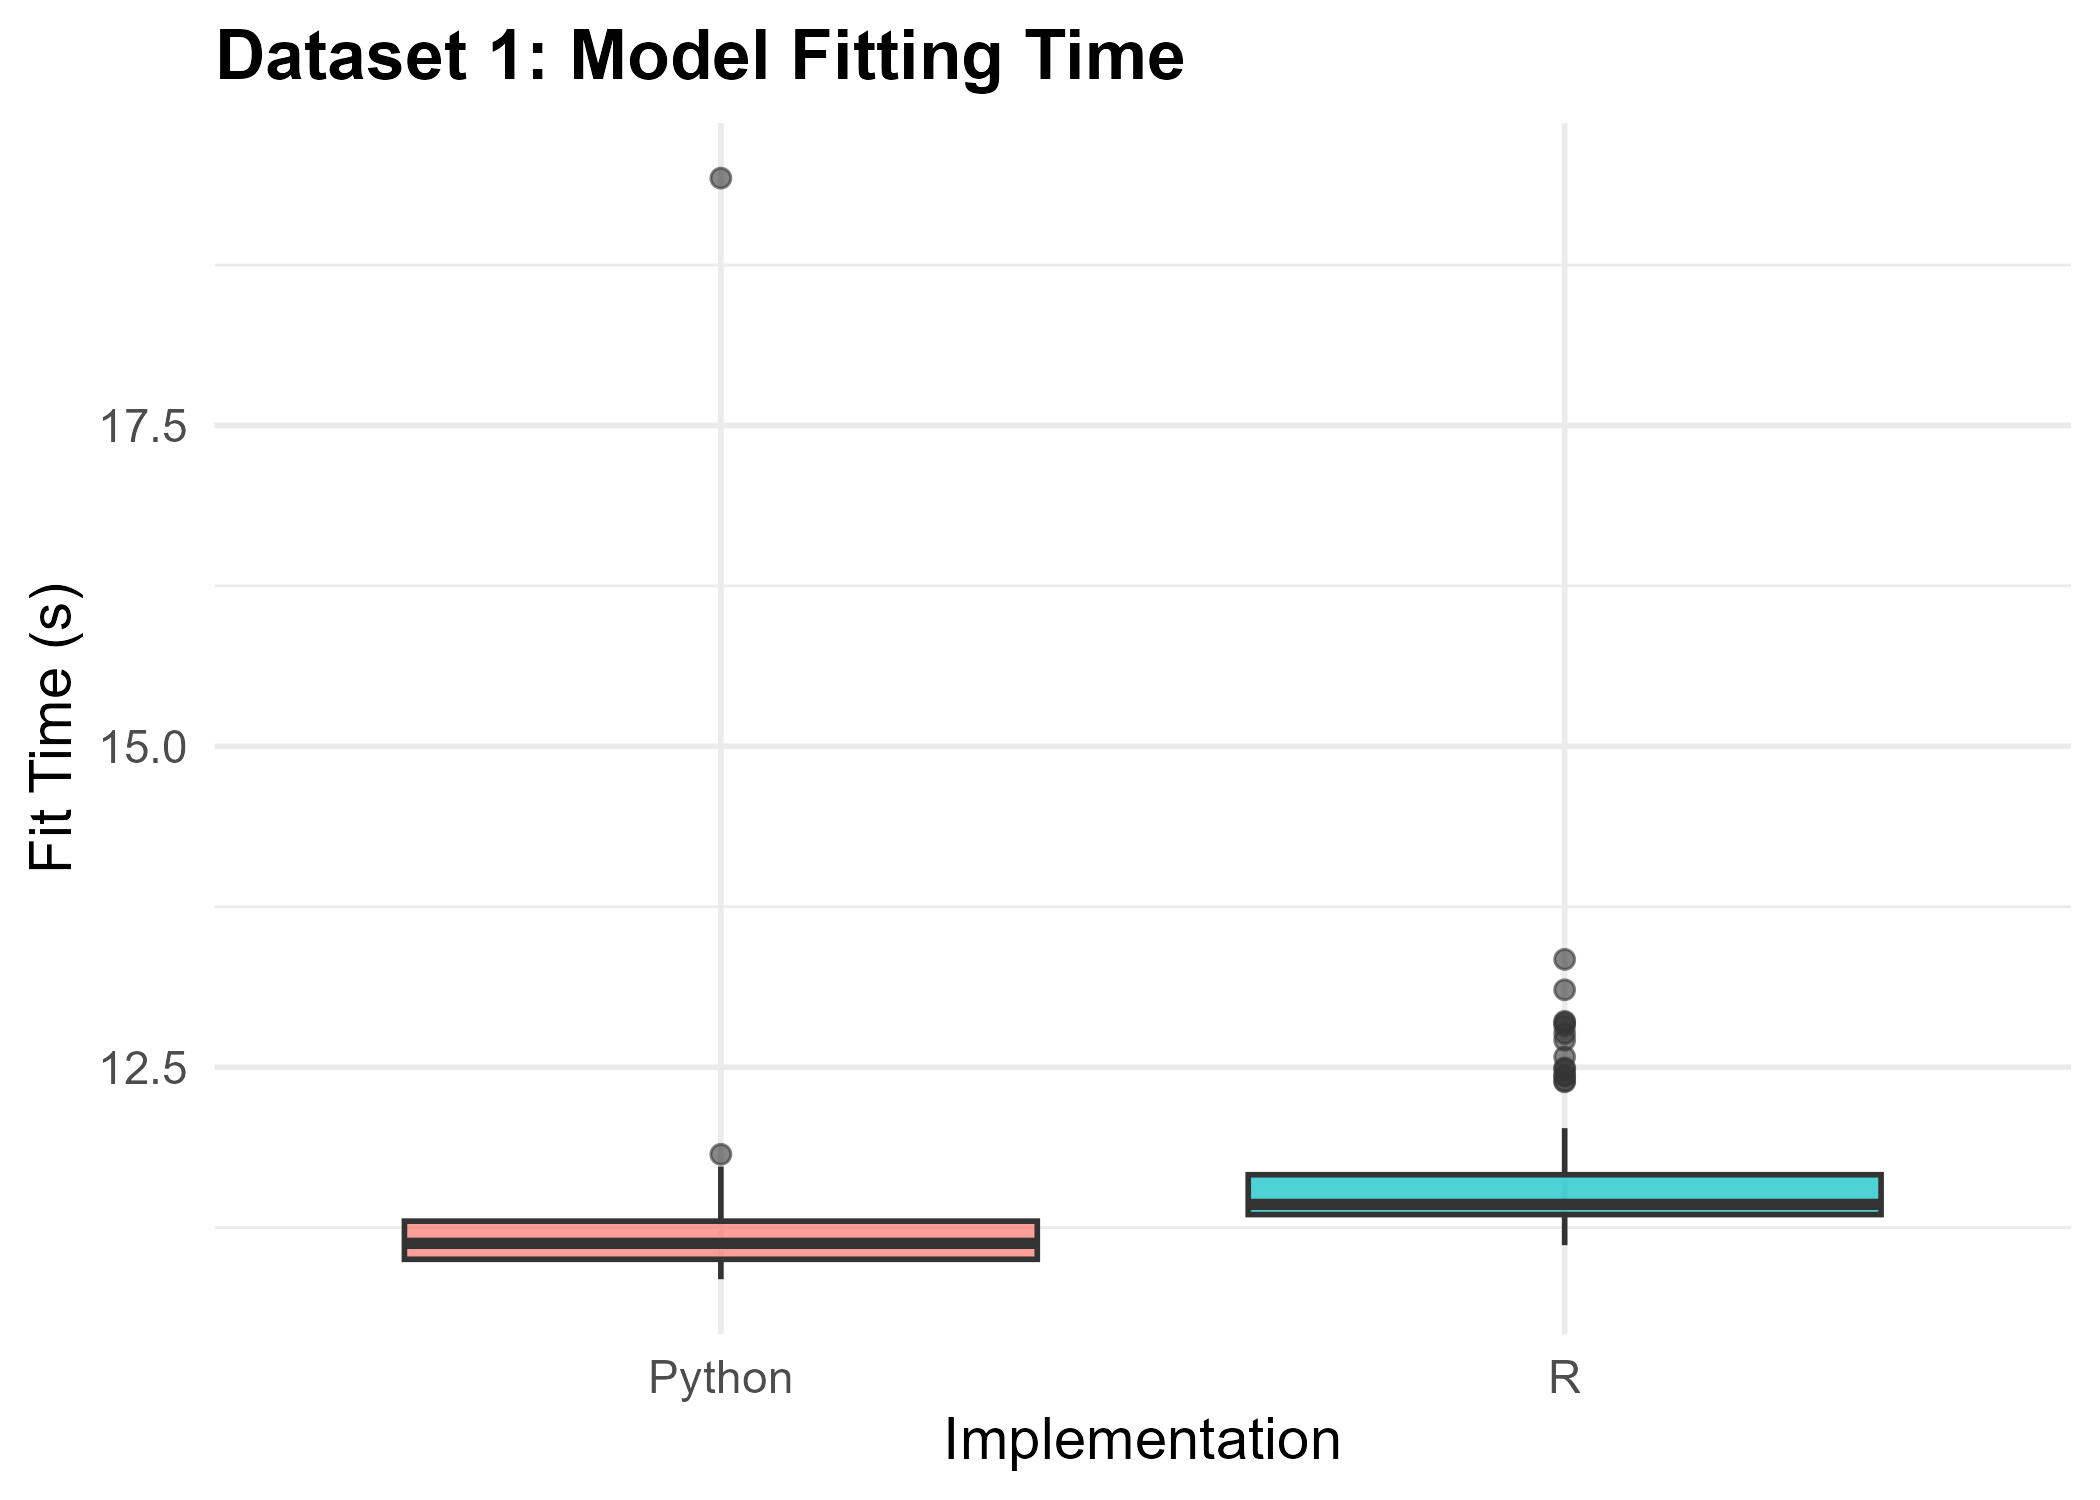
\includegraphics[width=\textwidth]{fit1.jpg}
    \caption{Fit 1}
\end{subfigure}
\begin{subfigure}{0.48\textwidth}
    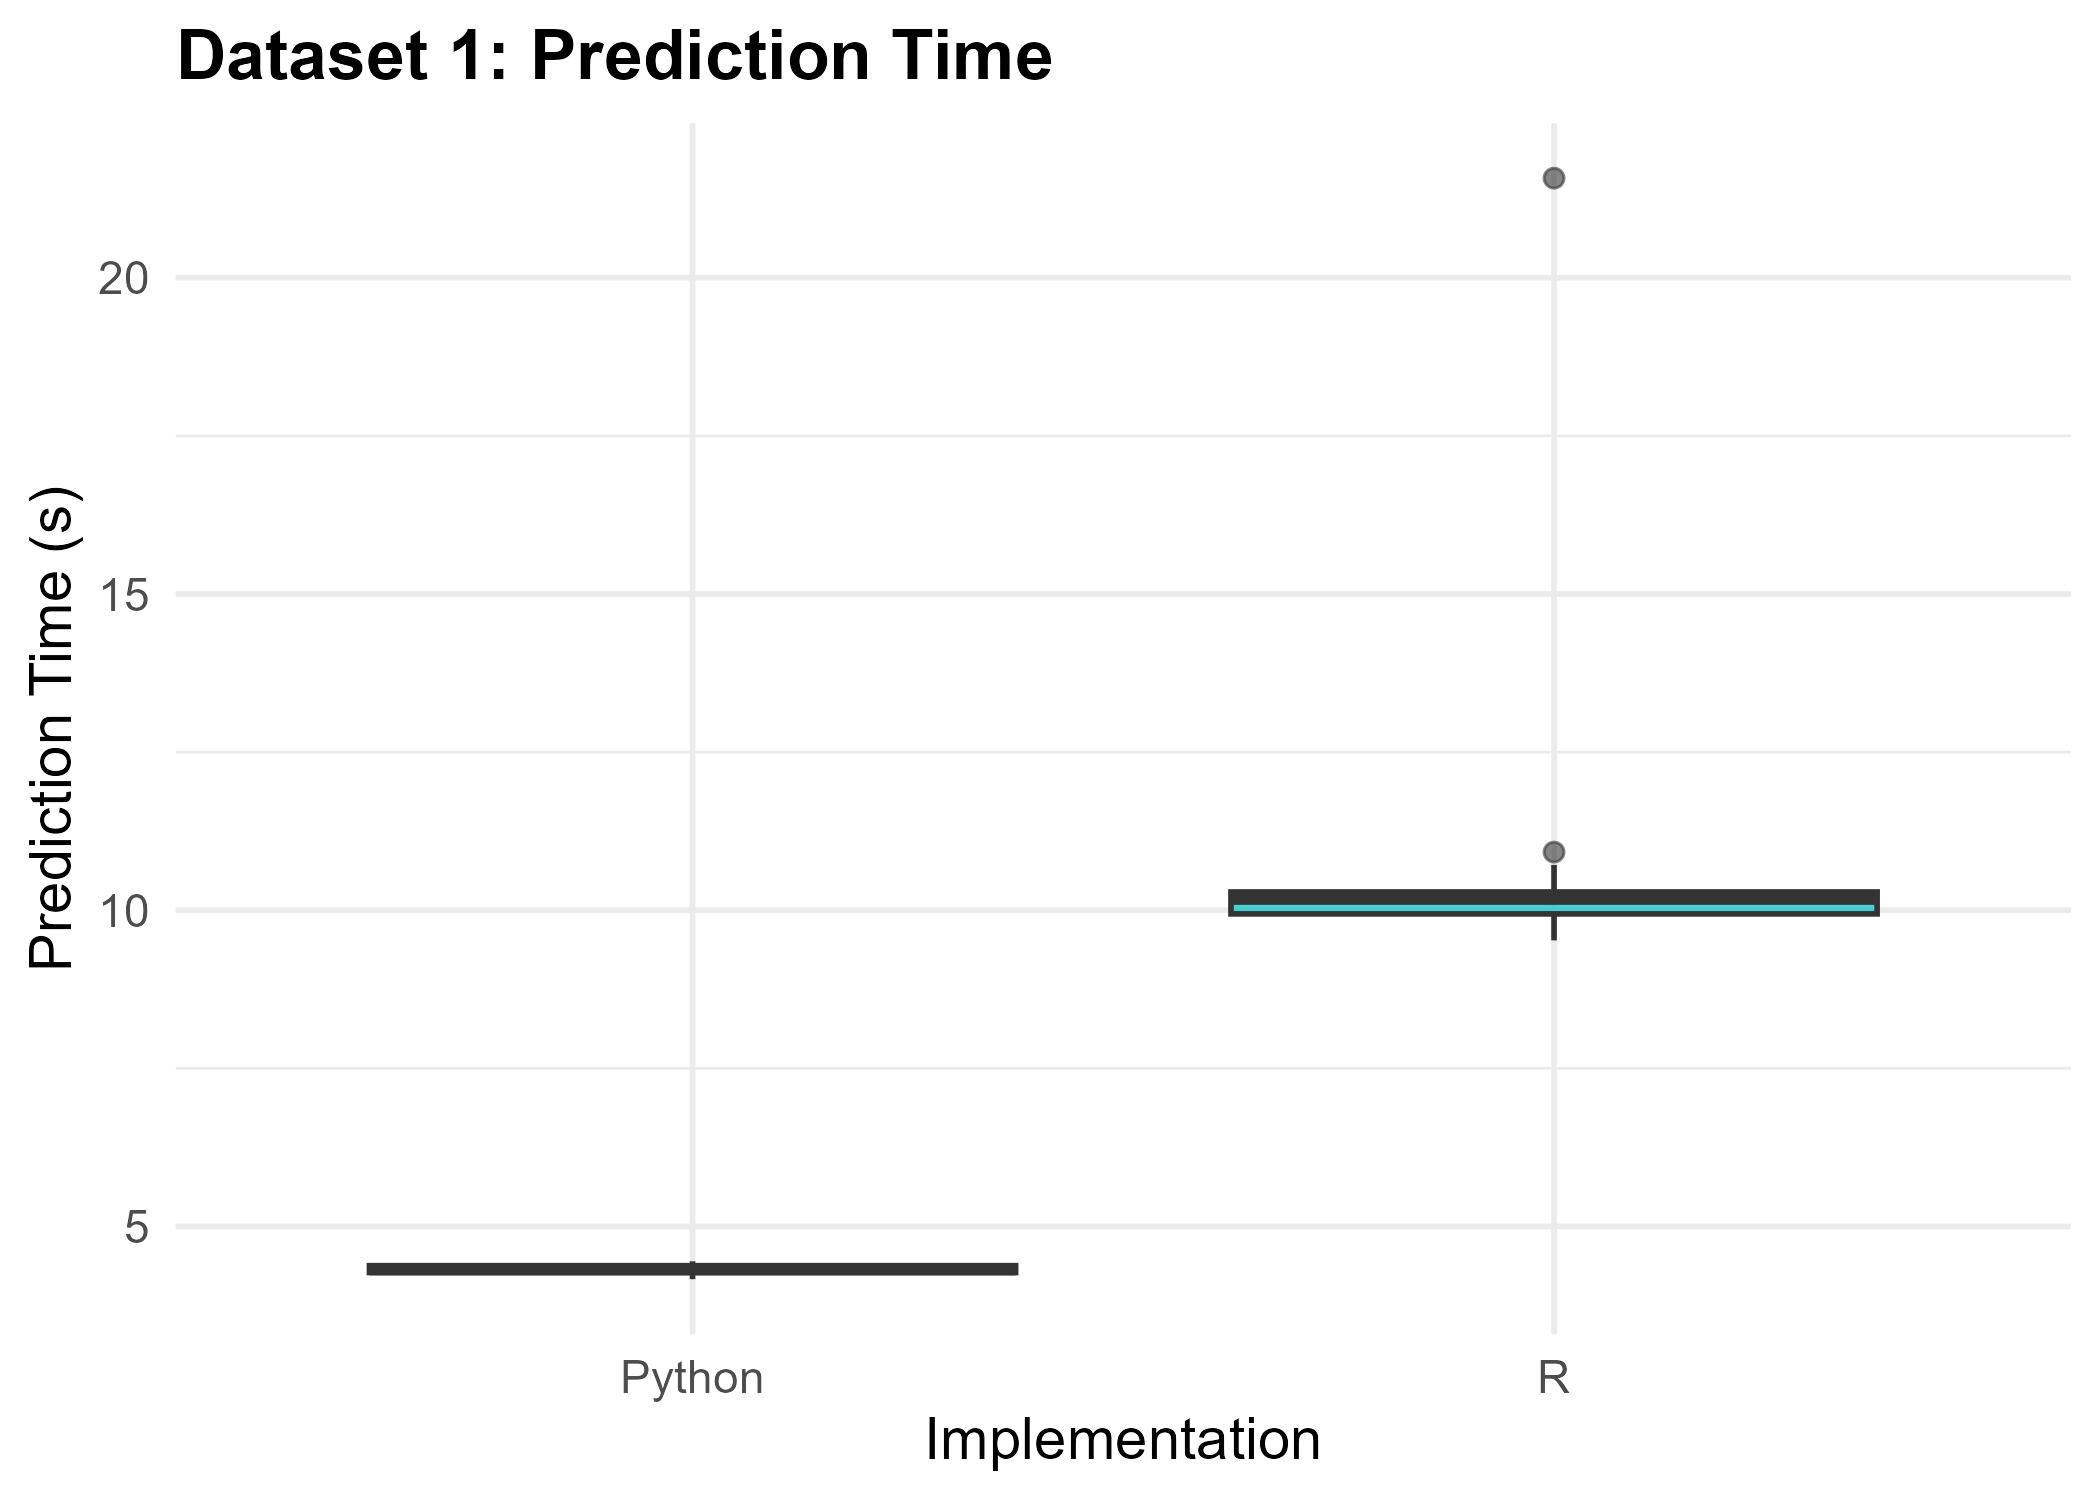
\includegraphics[width=\textwidth]{pred1.jpg}
    \caption{Pred 1}
\end{subfigure}

\vspace{0.3cm}

% Row 2 (Dataset 2)
\begin{subfigure}{0.48\textwidth}
    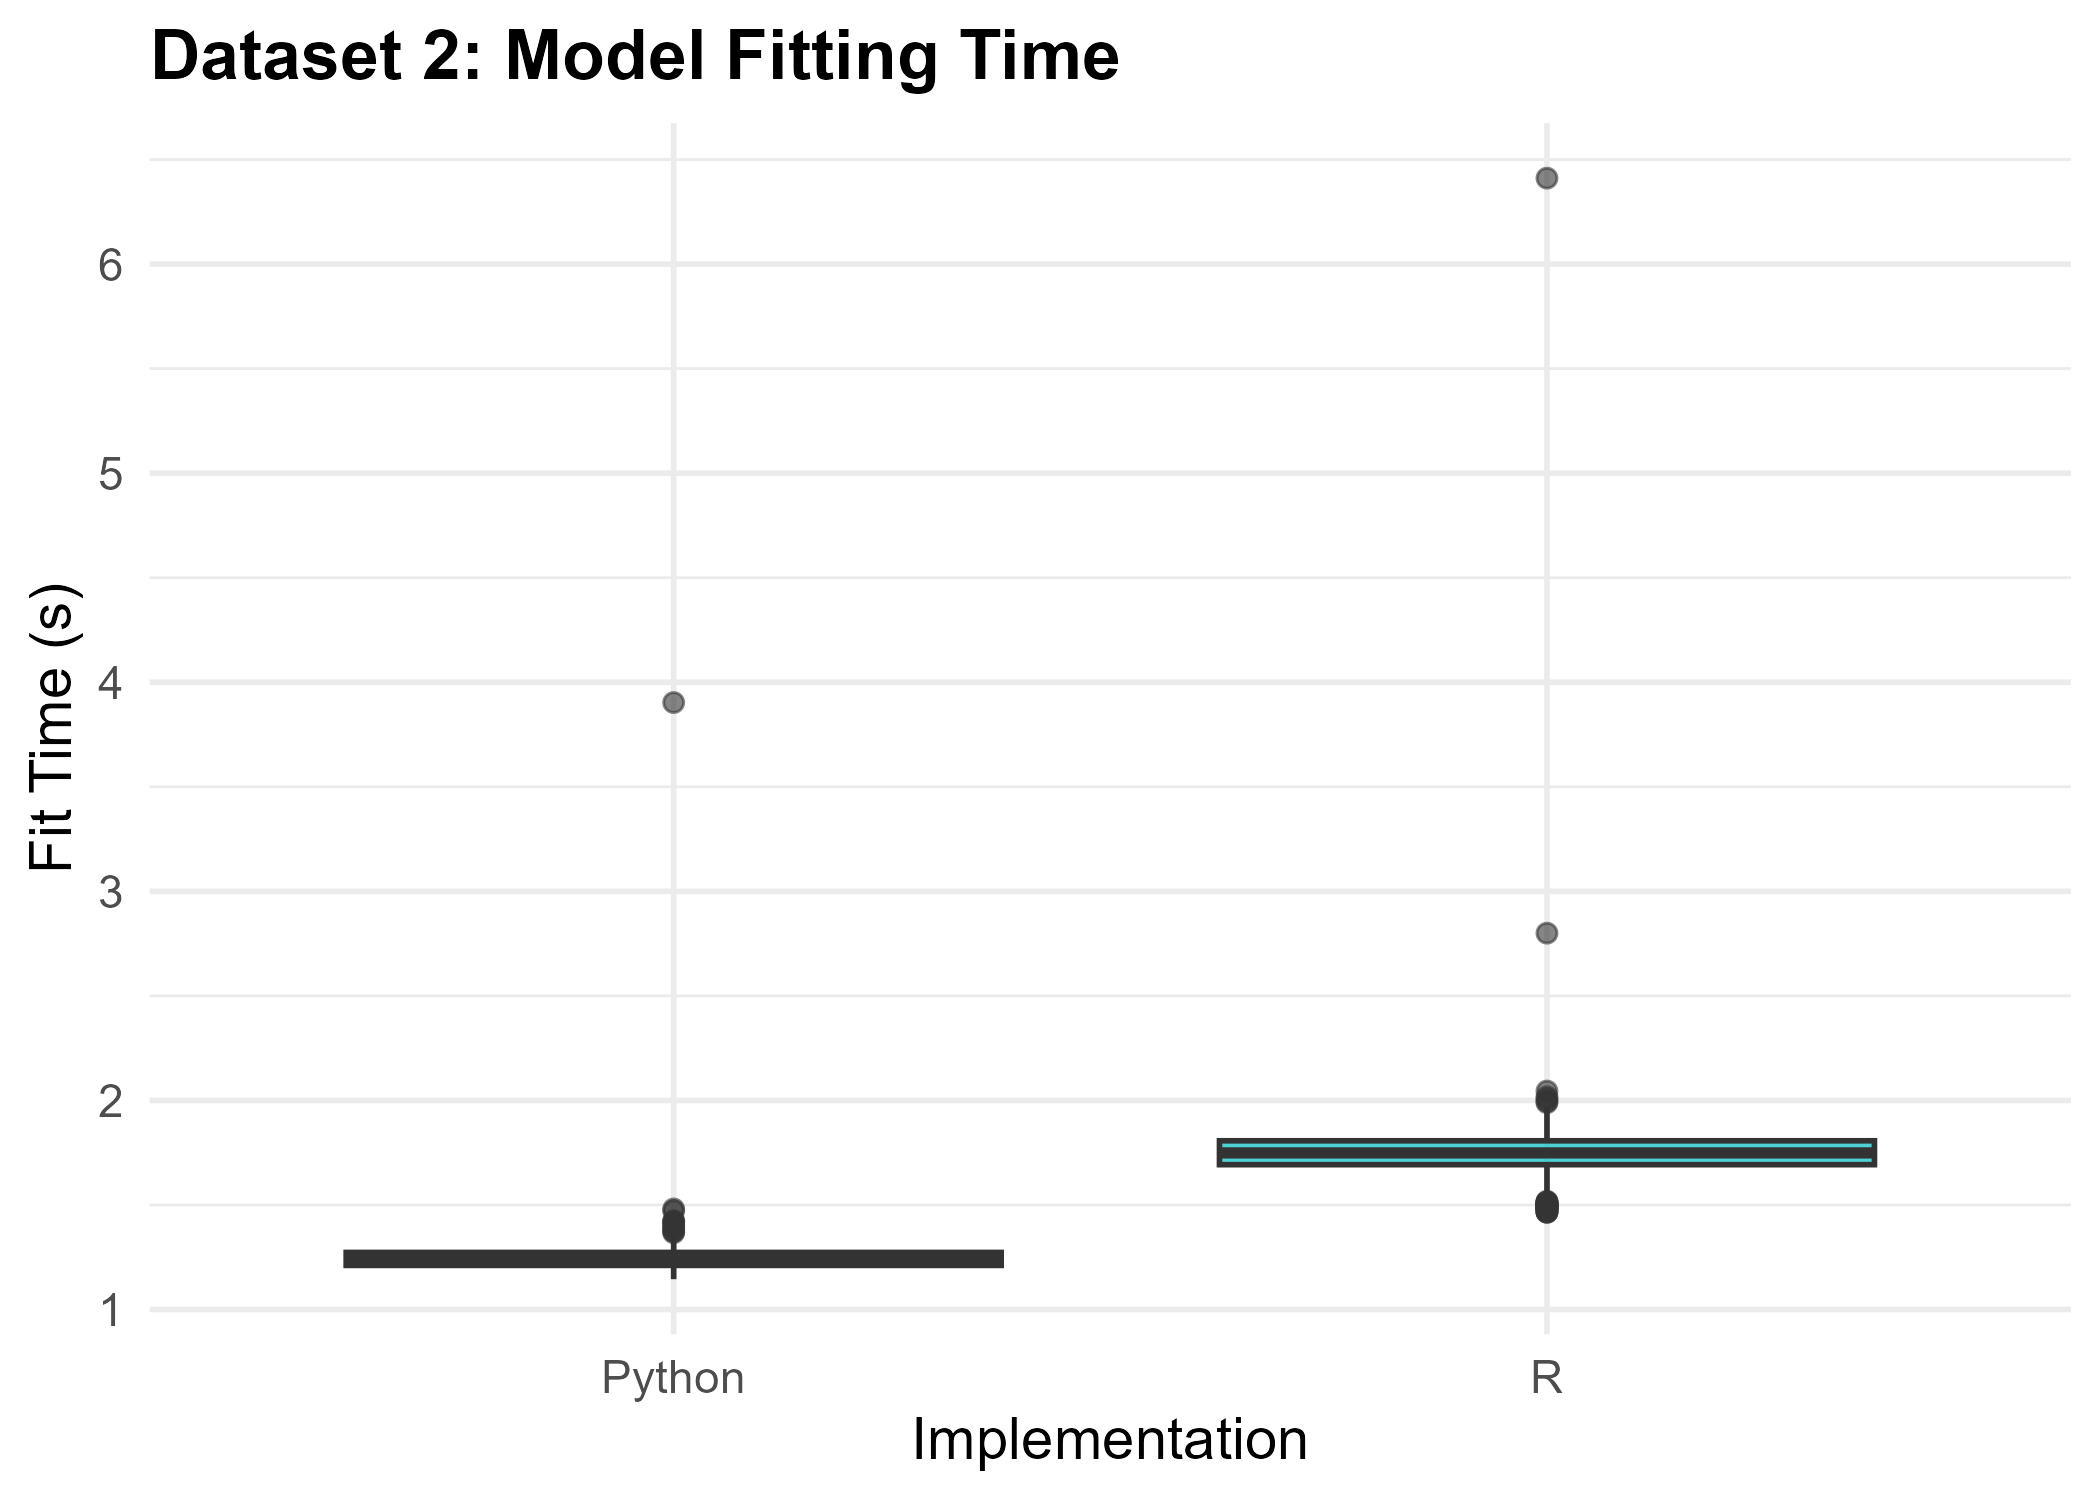
\includegraphics[width=\textwidth]{fit2.jpg}
    \caption{Fit 2}
\end{subfigure}
\begin{subfigure}{0.48\textwidth}
    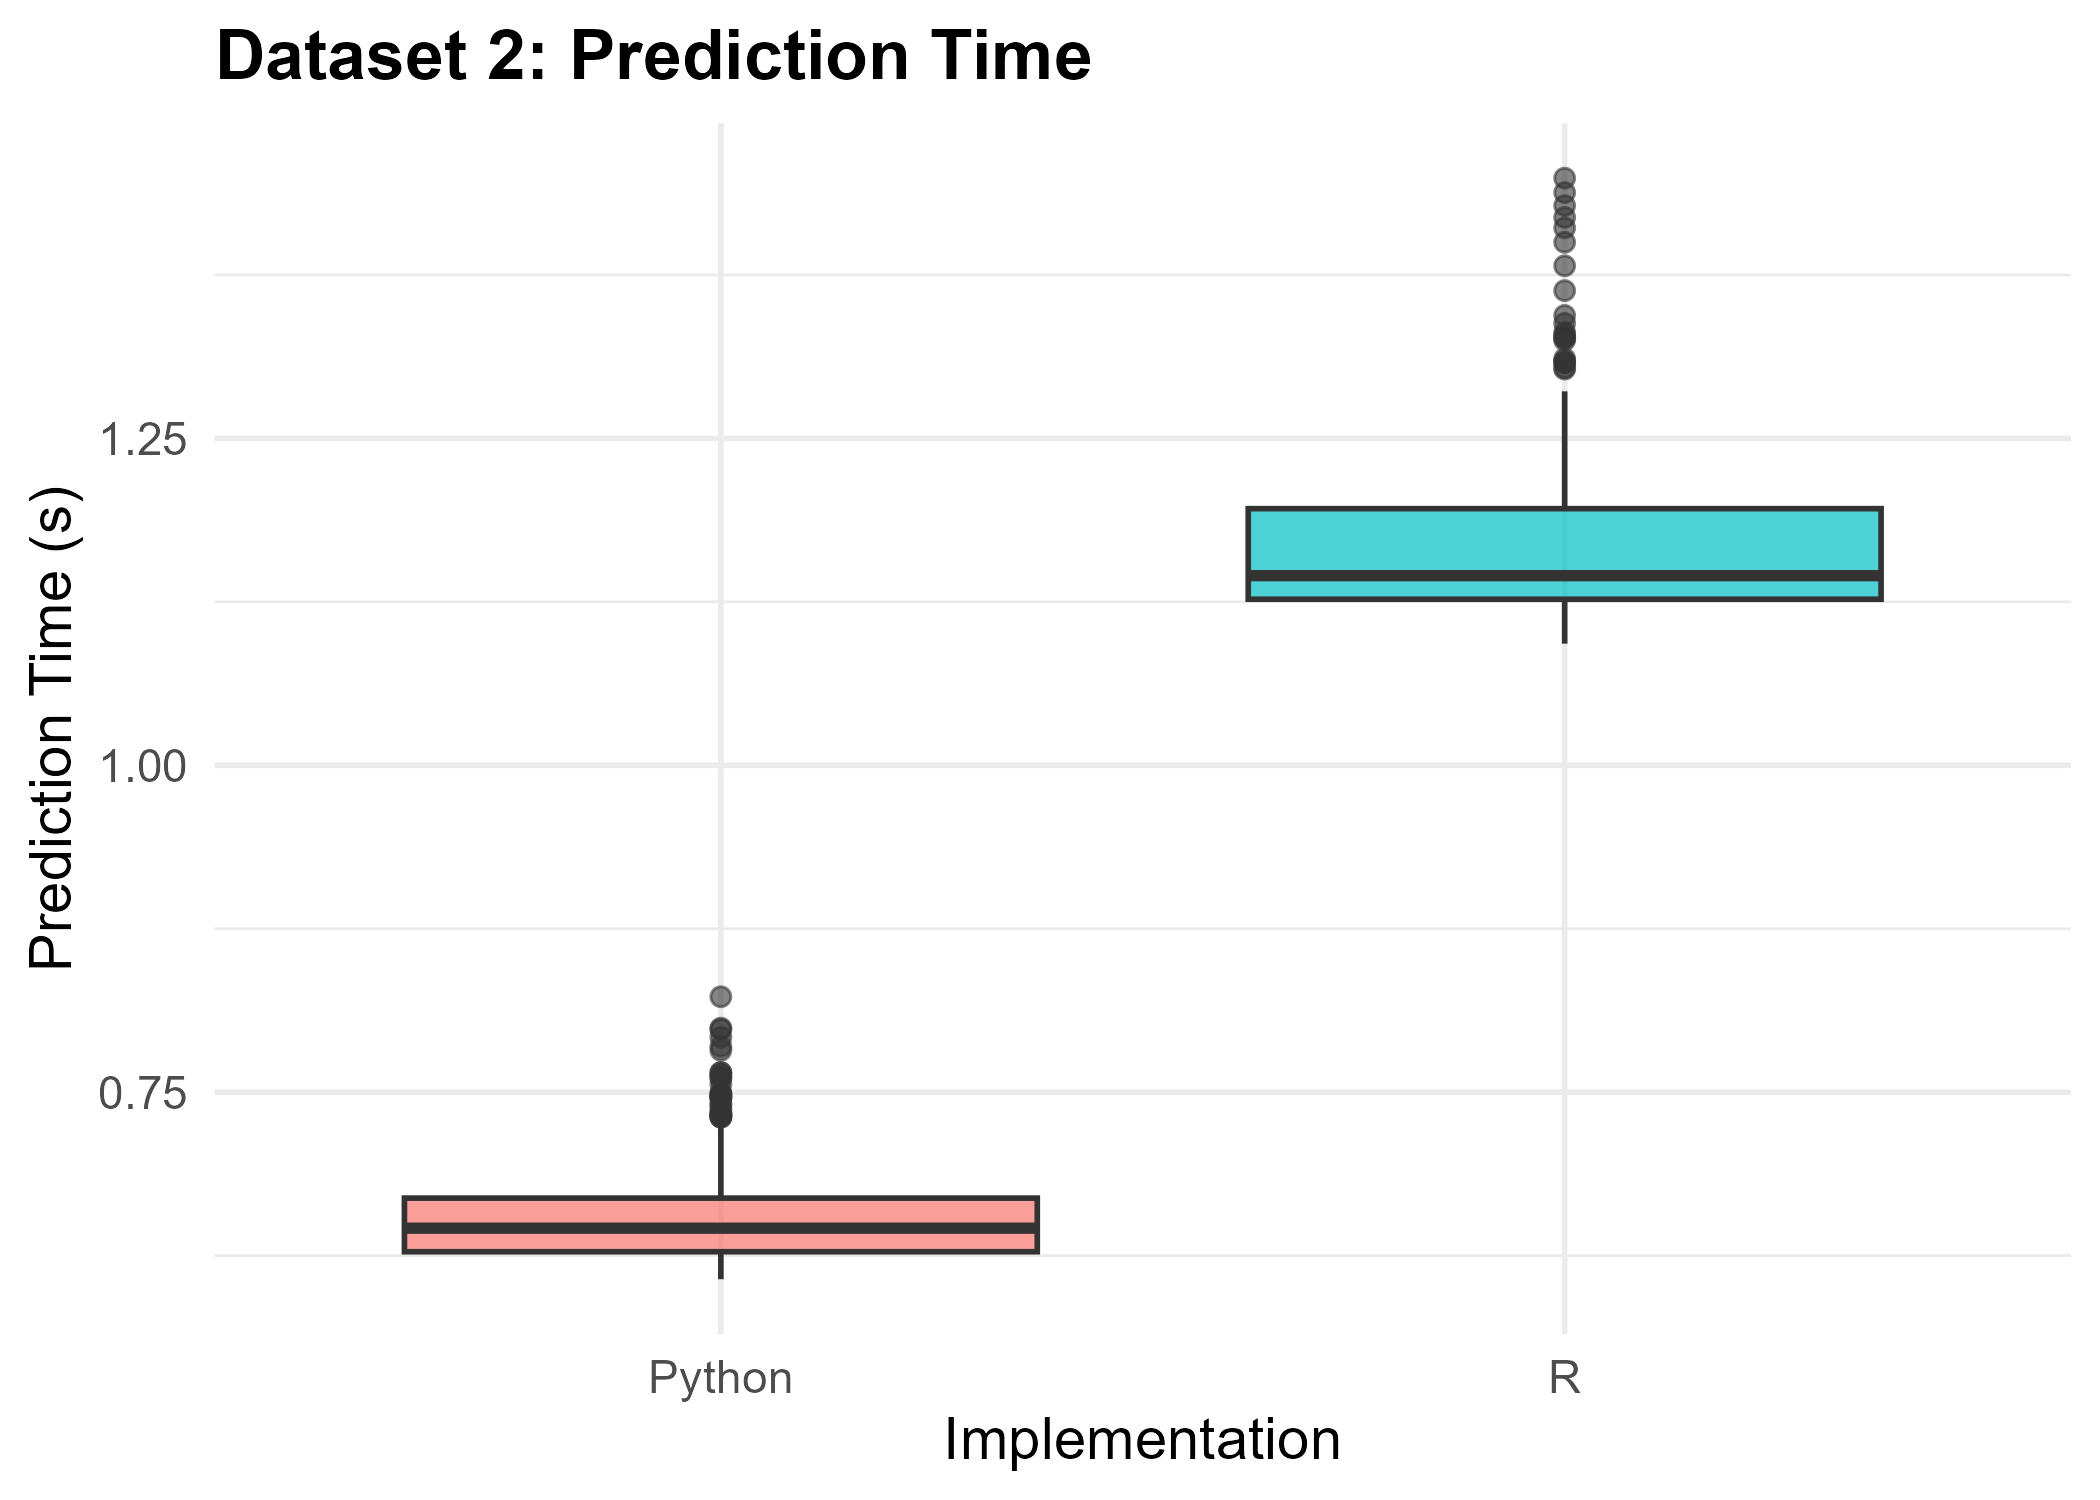
\includegraphics[width=\textwidth]{pred2.jpg}
    \caption{Pred 2}
\end{subfigure}

\vspace{0.3cm}

% Row 3 (Dataset 3)
\begin{subfigure}{0.48\textwidth}
    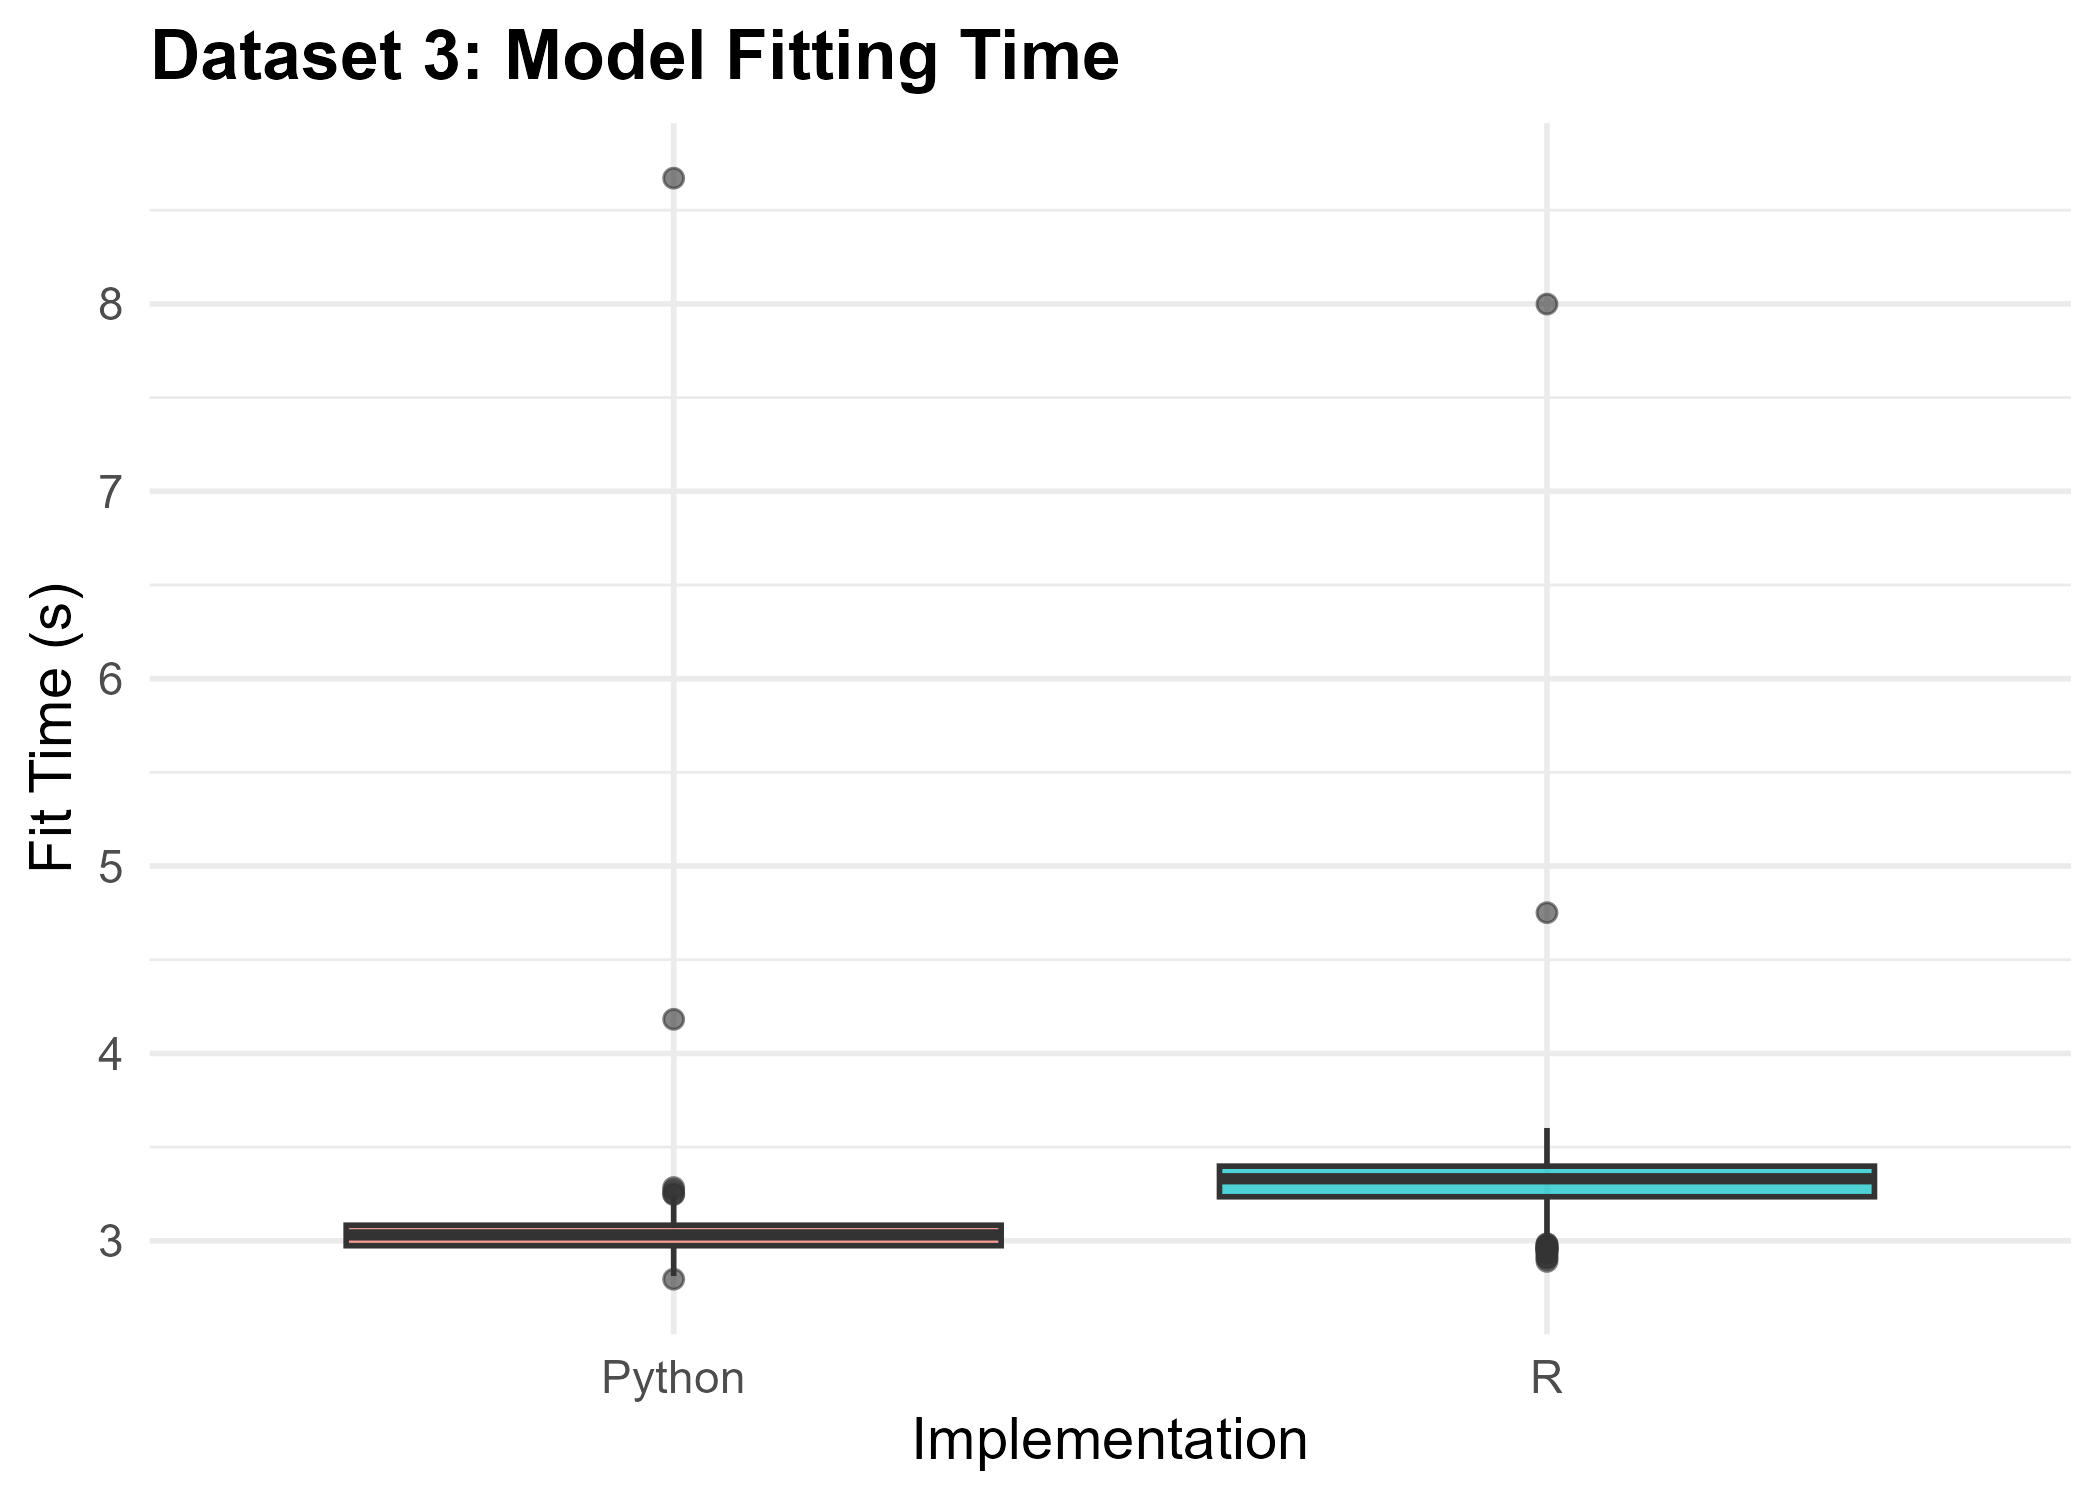
\includegraphics[width=\textwidth]{fit3.jpg}
    \caption{Fit 3}
\end{subfigure}
\begin{subfigure}{0.48\textwidth}
    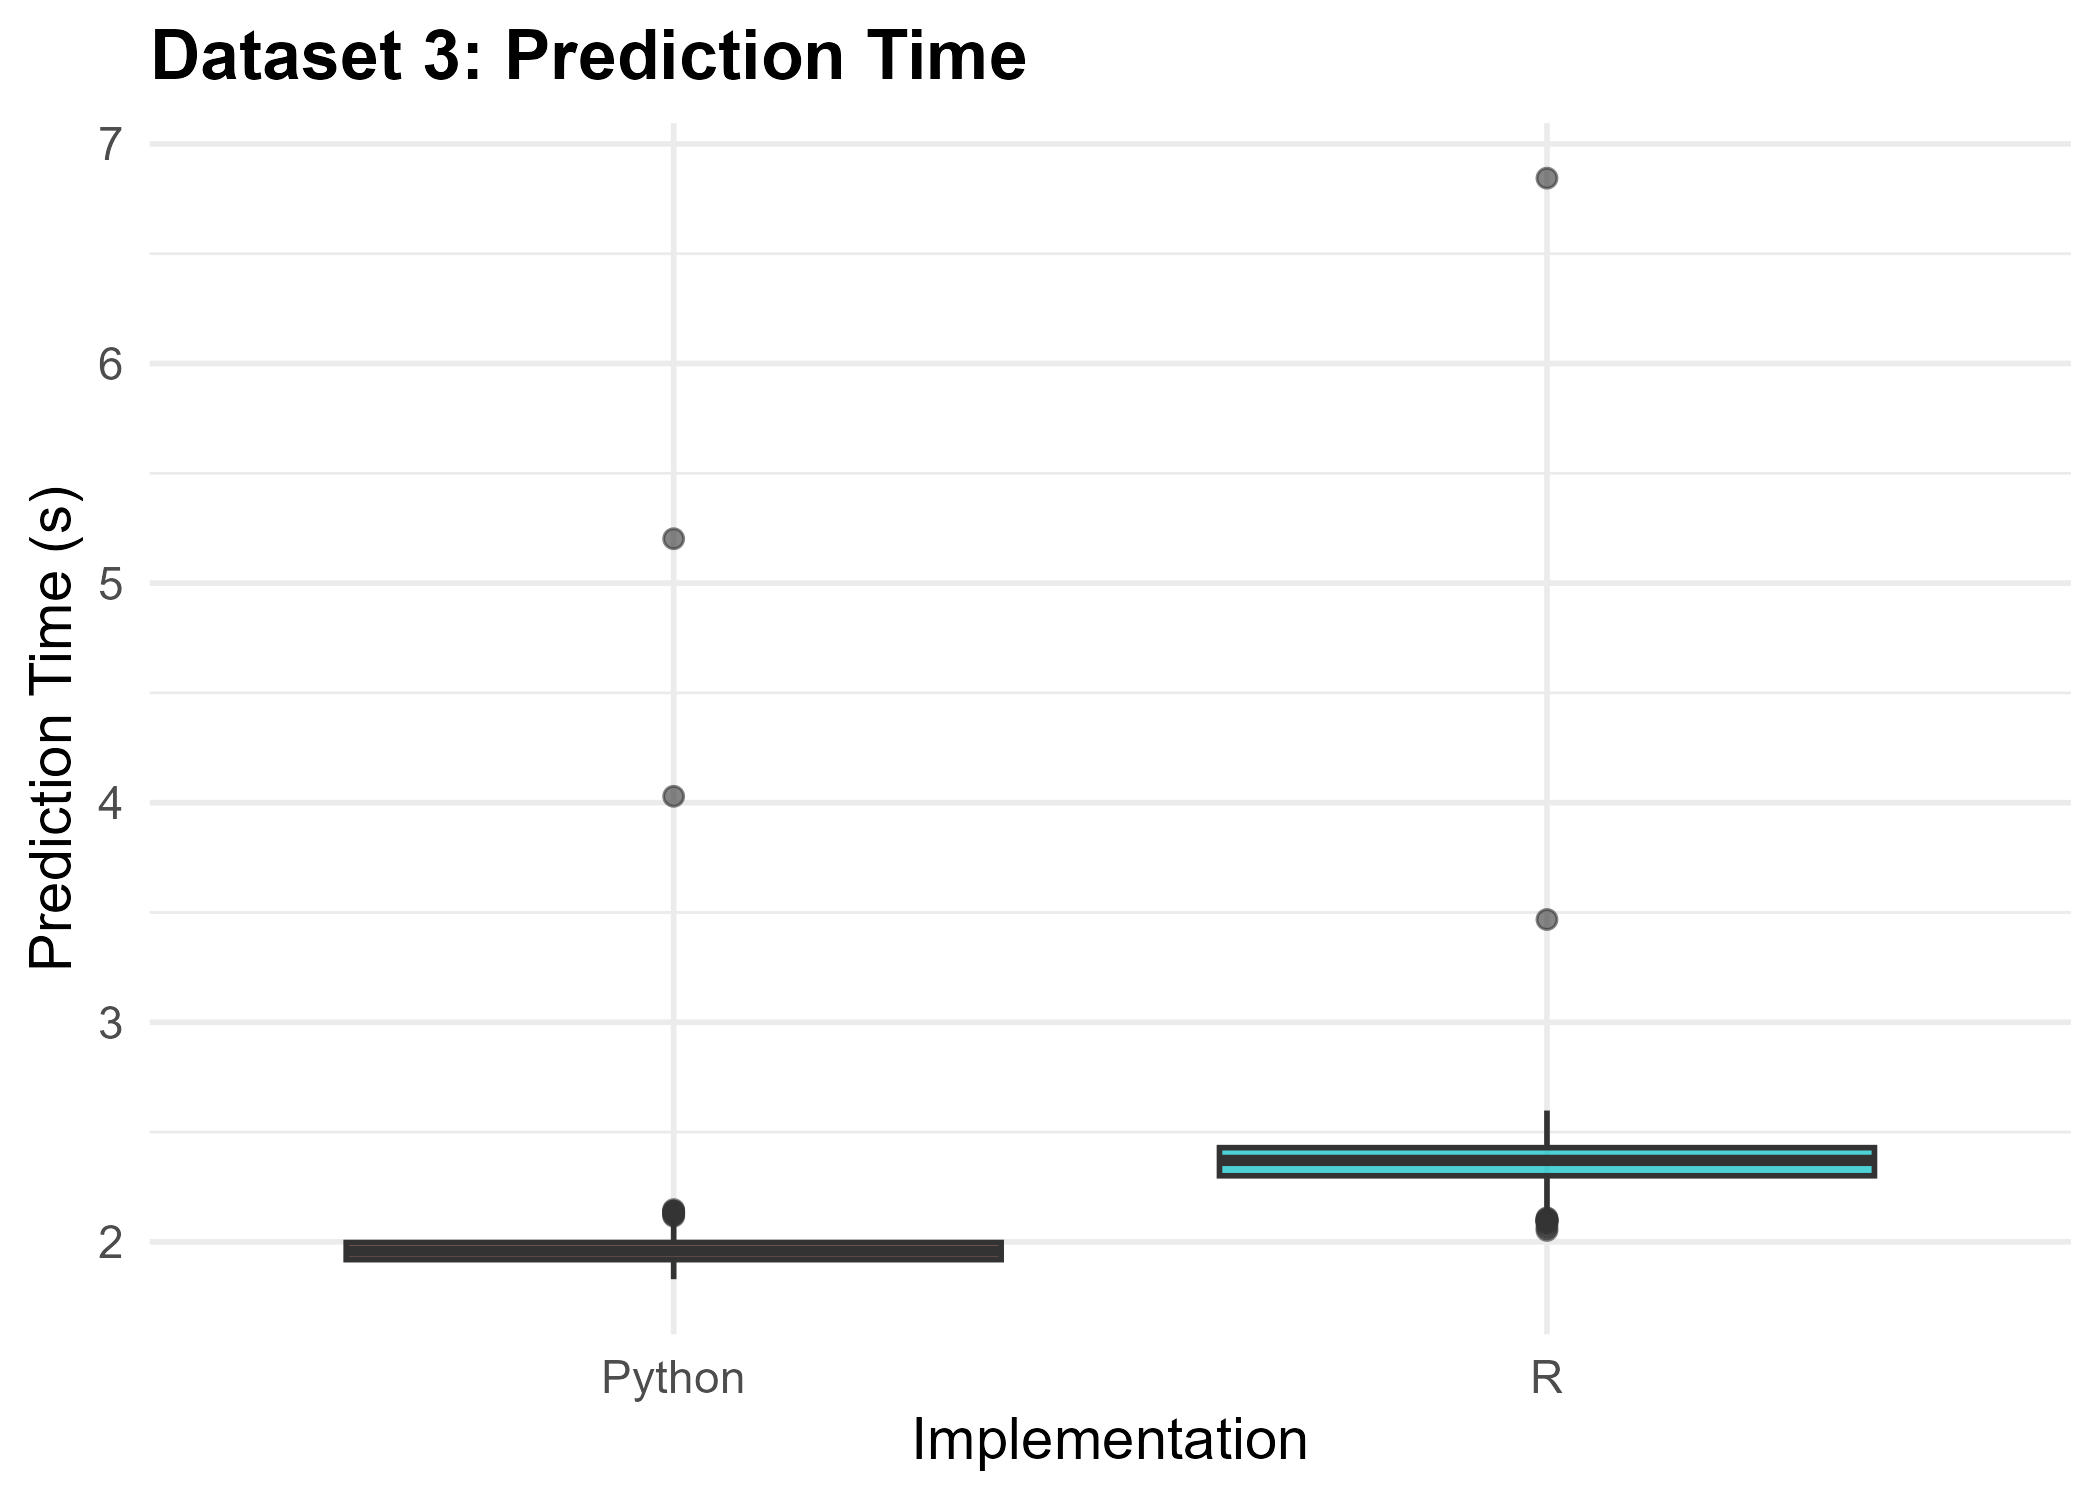
\includegraphics[width=\textwidth]{pred3.jpg}
    \caption{Pred 3}
\end{subfigure}

\vspace{0.3cm}

% Row 4 (Dataset 4)
\begin{subfigure}{0.48\textwidth}
    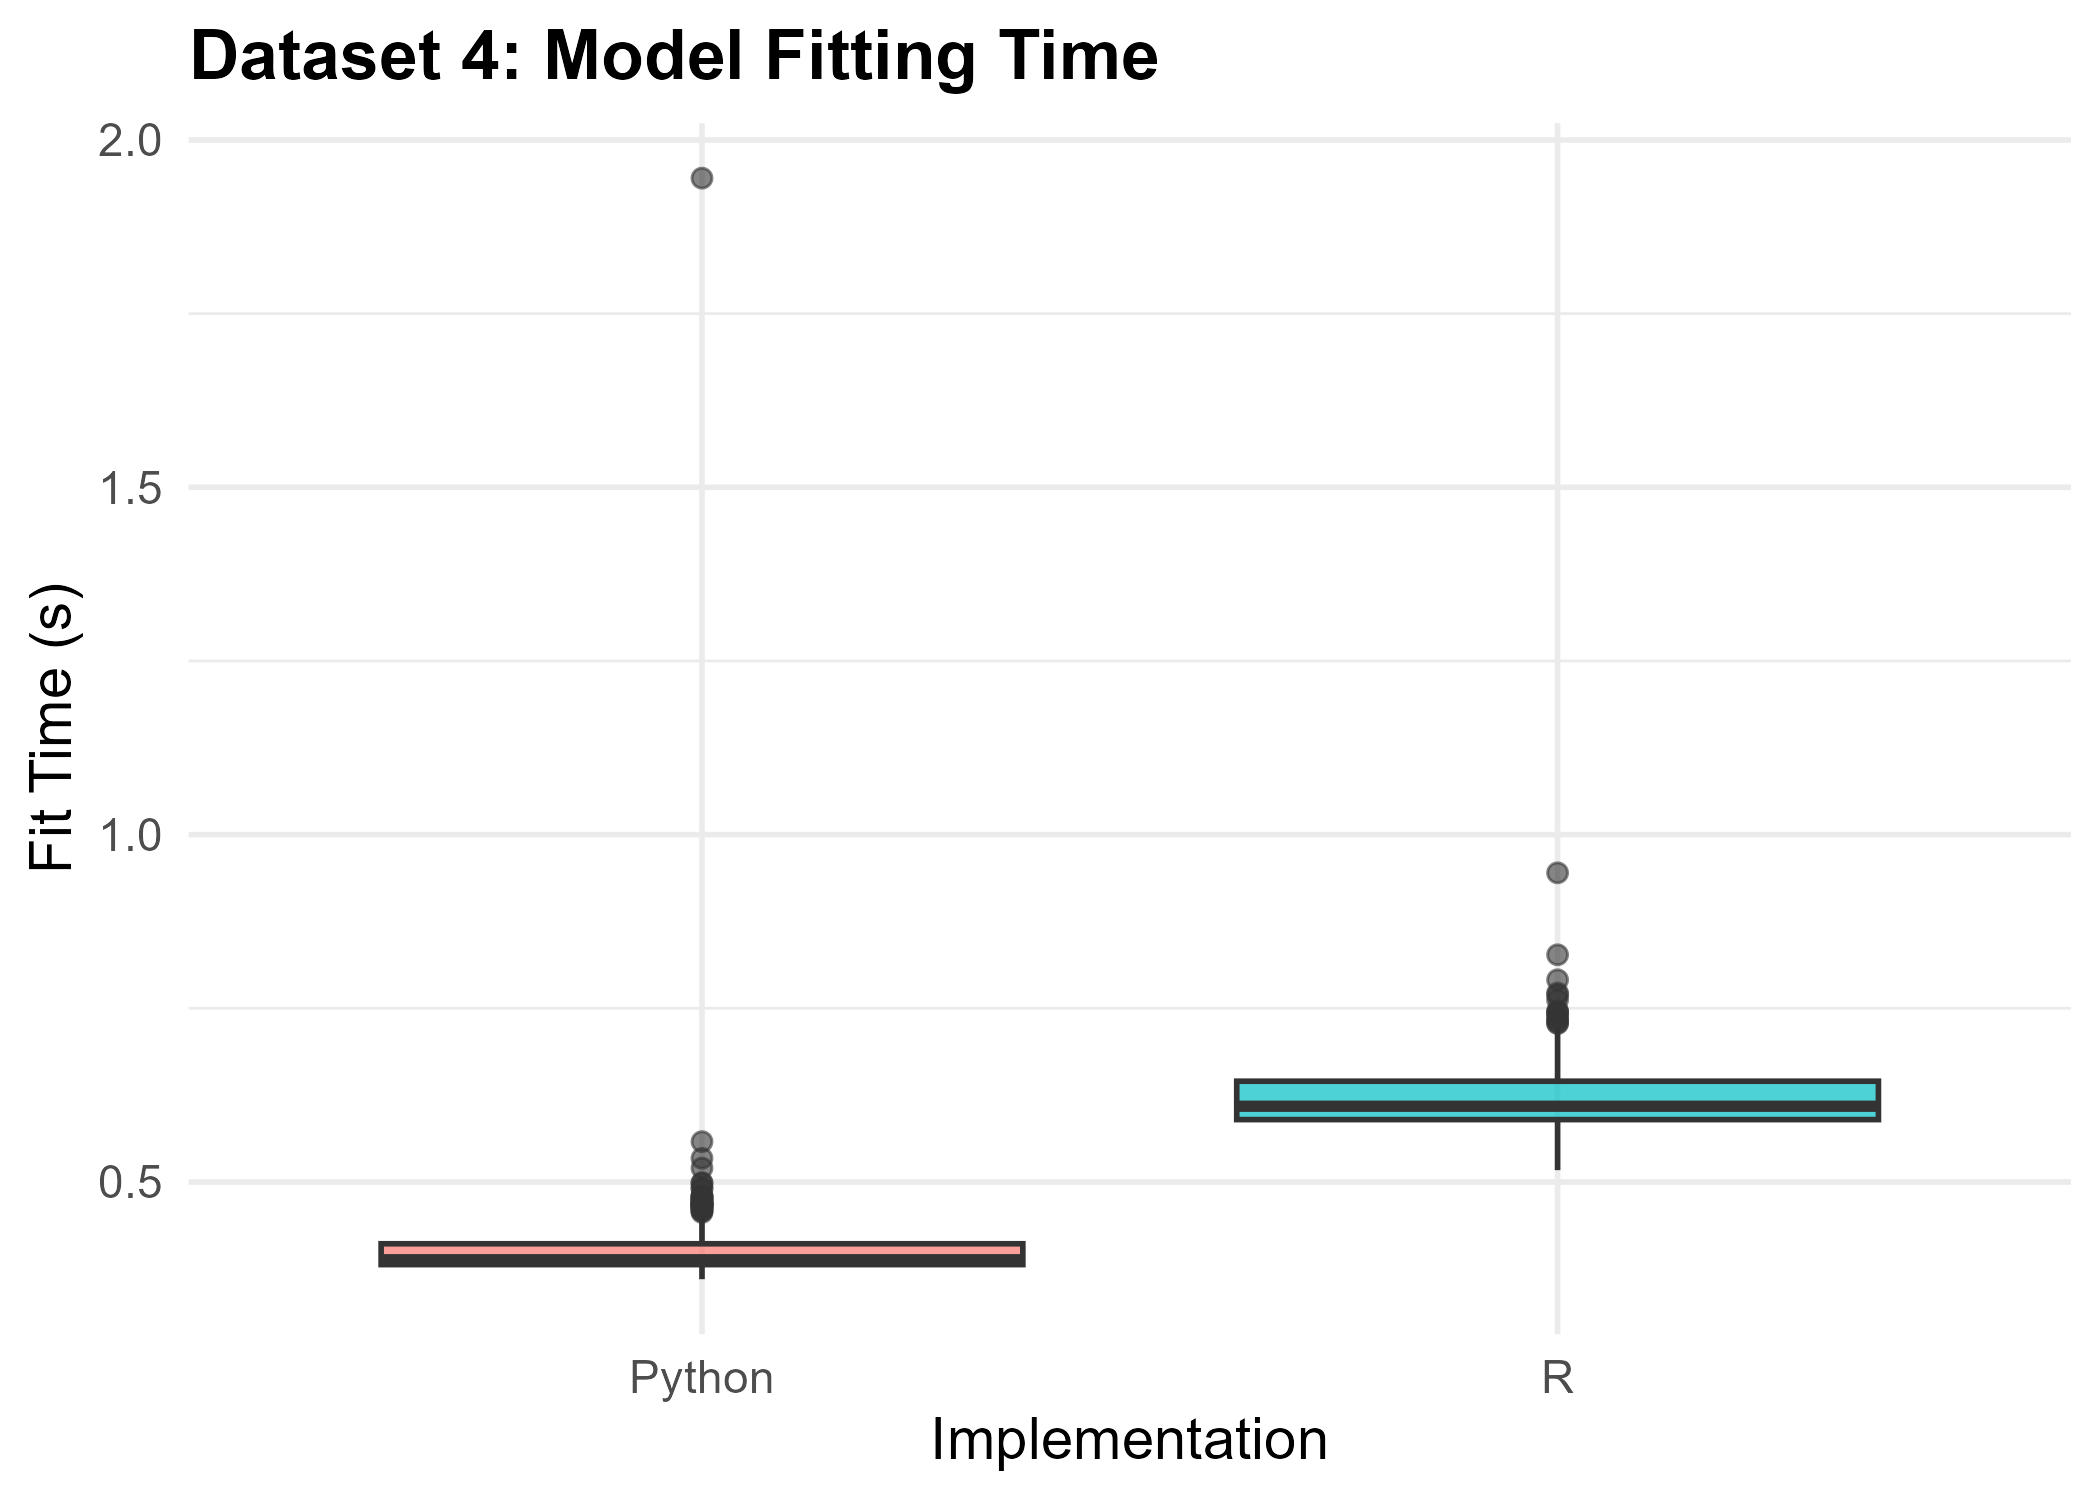
\includegraphics[width=\textwidth]{fit4.jpg}
    \caption{Fit 4}
\end{subfigure}
\begin{subfigure}{0.48\textwidth}
    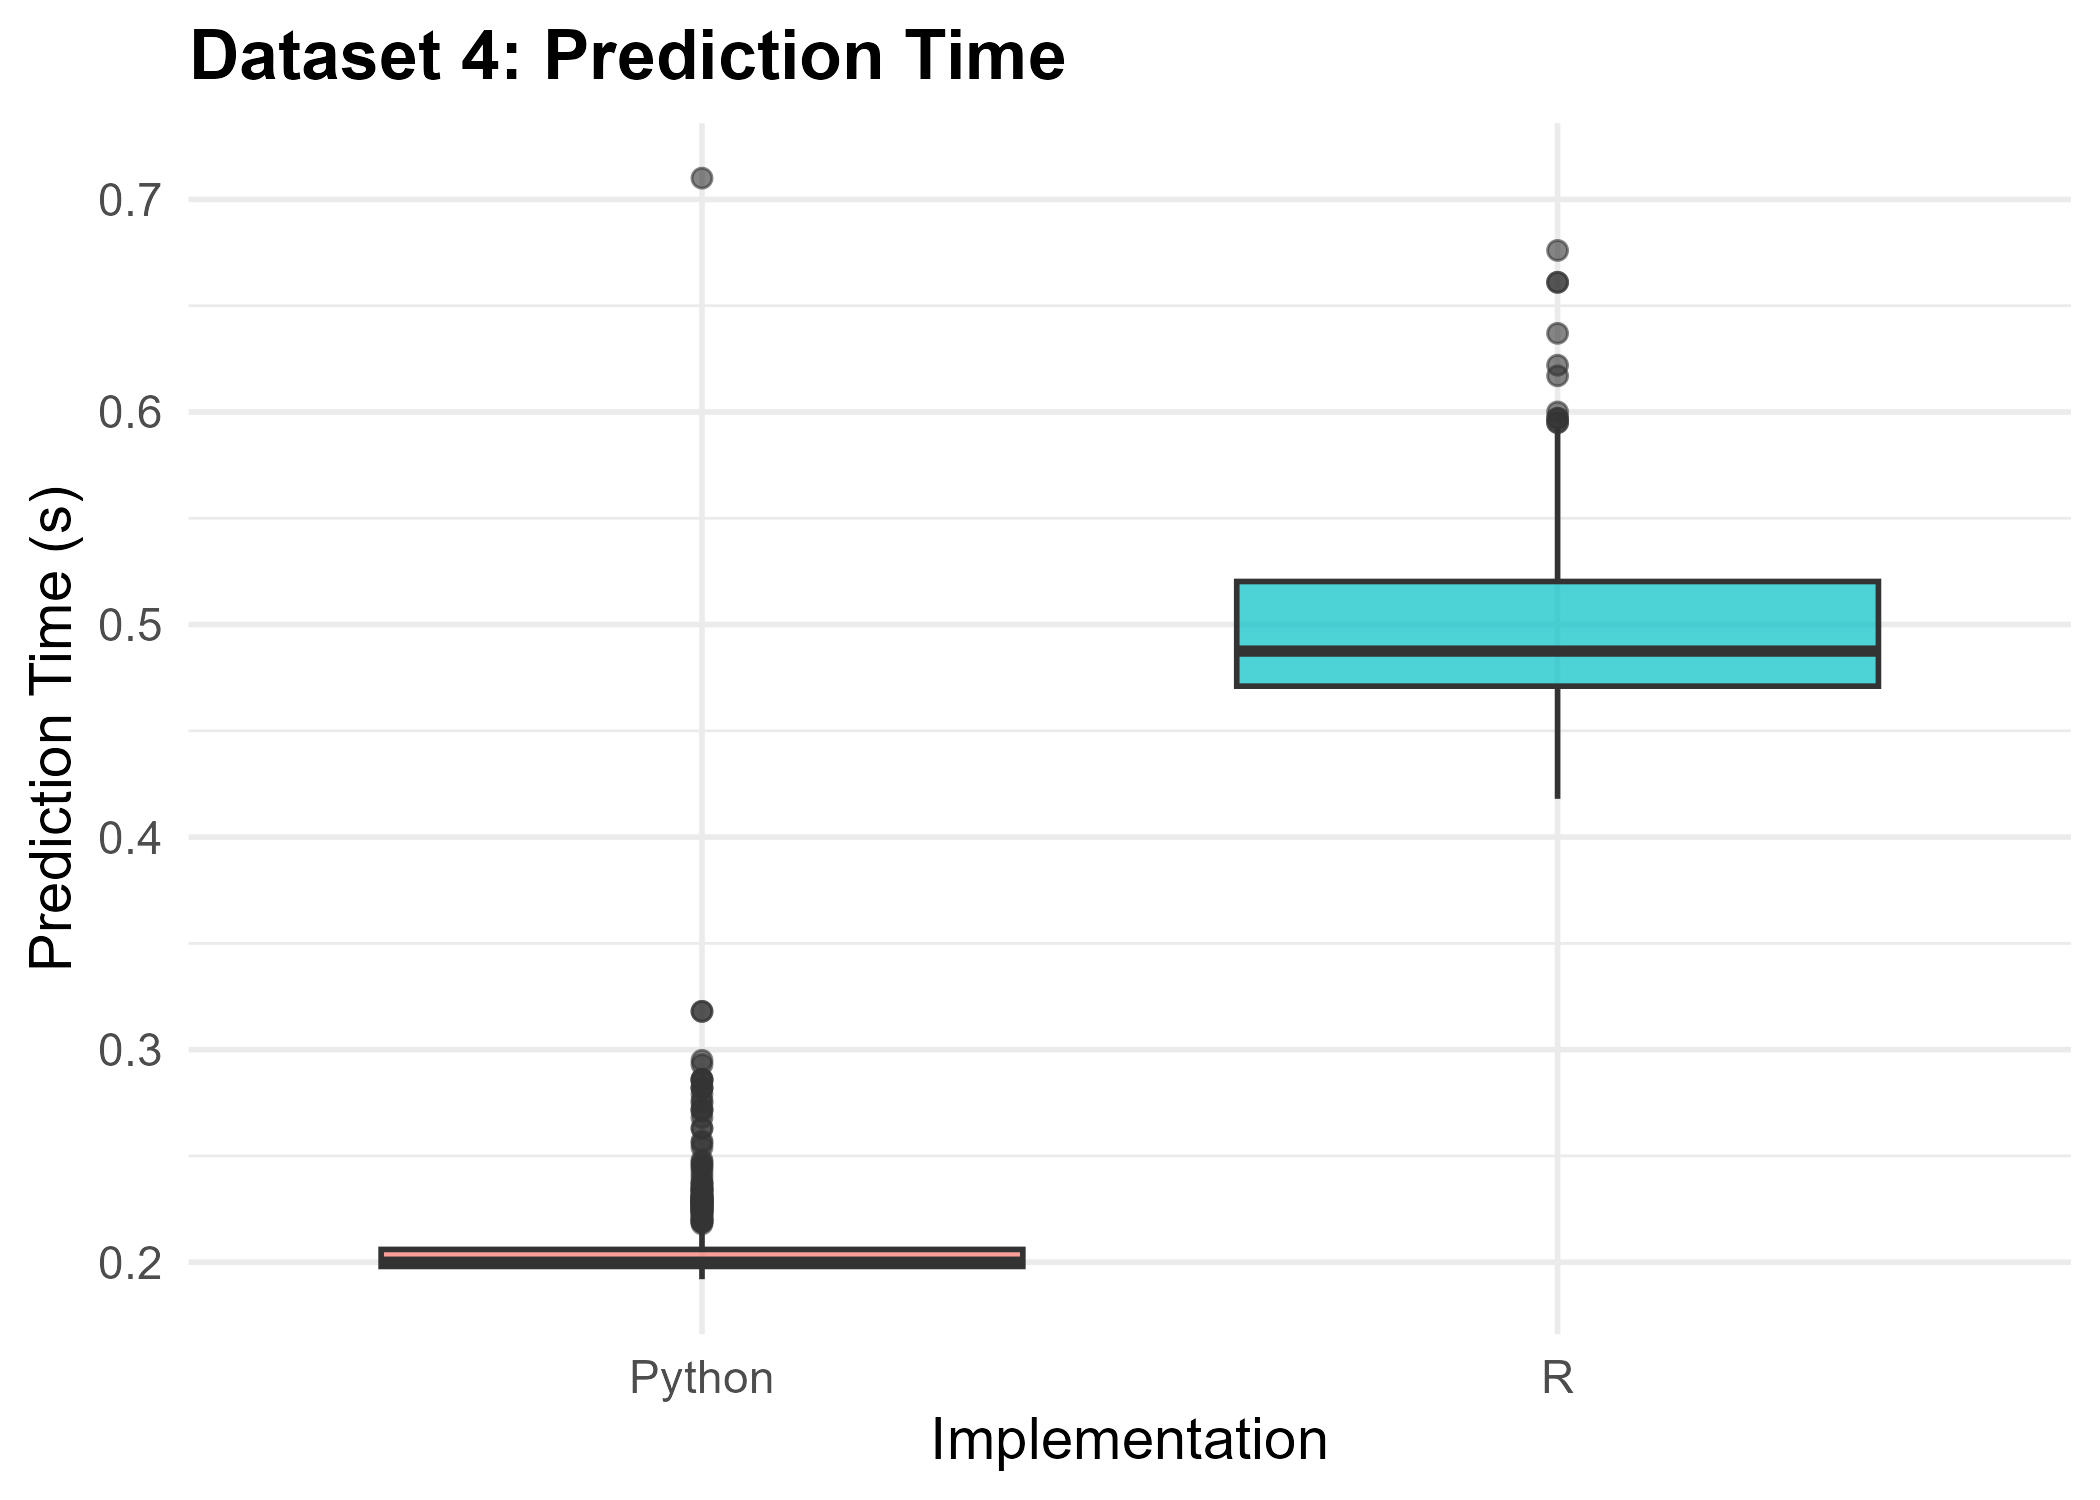
\includegraphics[width=\textwidth]{pred4.jpg}
    \caption{Pred 4}
\end{subfigure}

\caption{Model fitting and prediction times across datasets.}
\end{figure}

\begin{figure}[H]
\centering

% Row 1 (Dataset 1)
\begin{subfigure}{0.48\textwidth}
    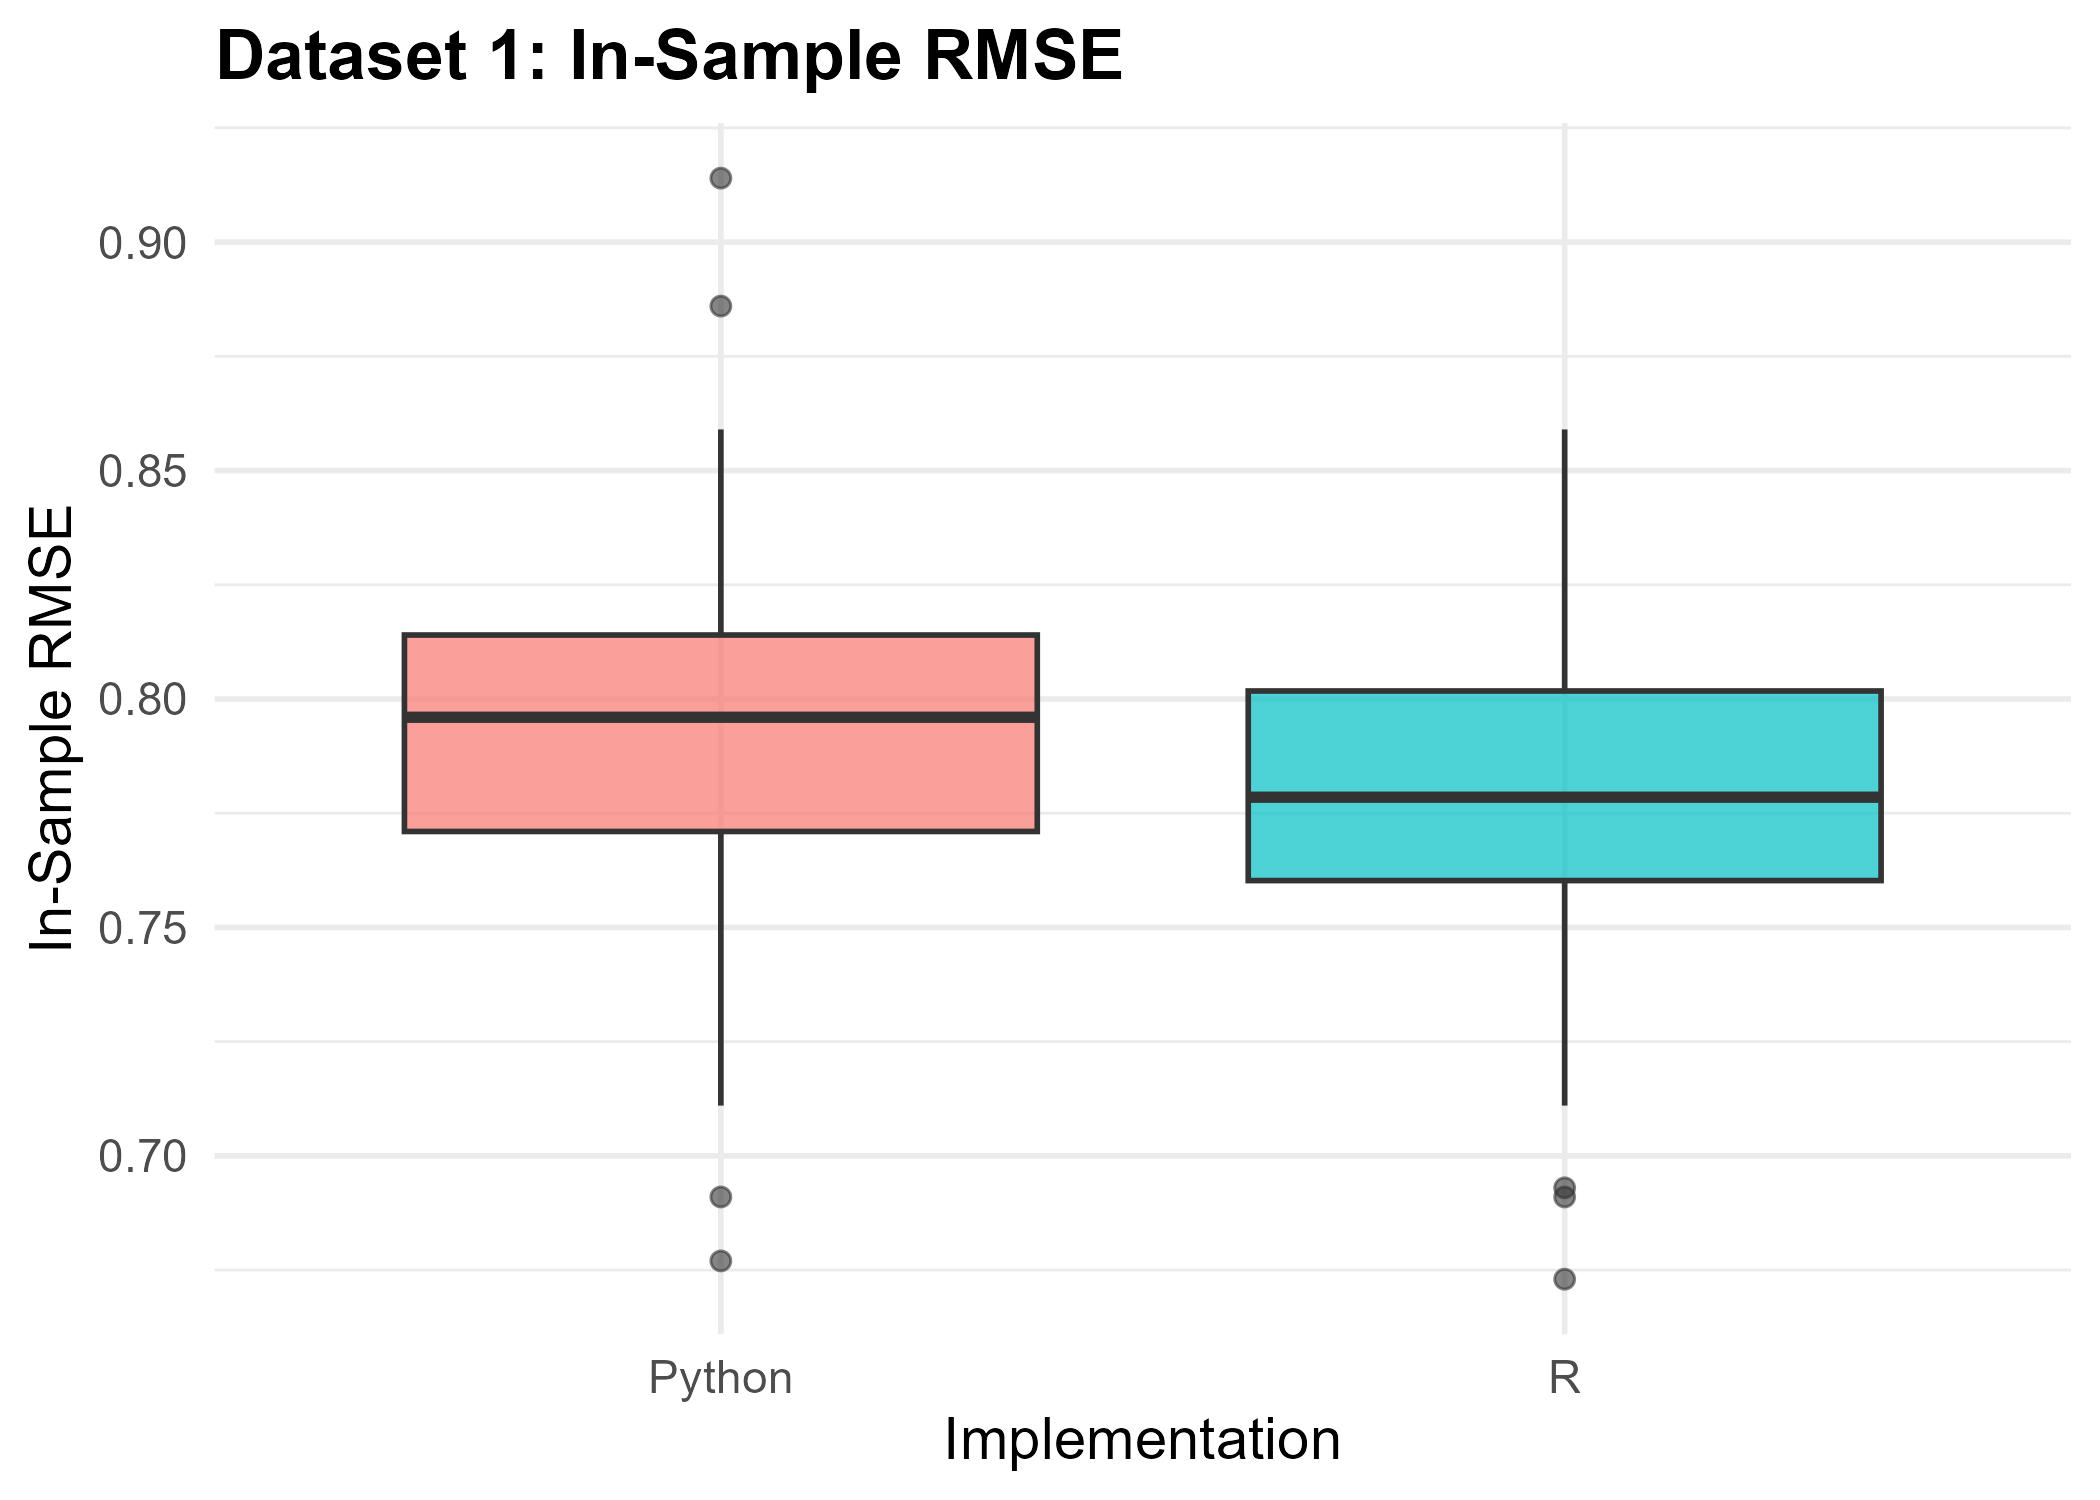
\includegraphics[width=\textwidth]{irmse1.jpg}
    \caption{iRMSE 1}
\end{subfigure}
\begin{subfigure}{0.48\textwidth}
    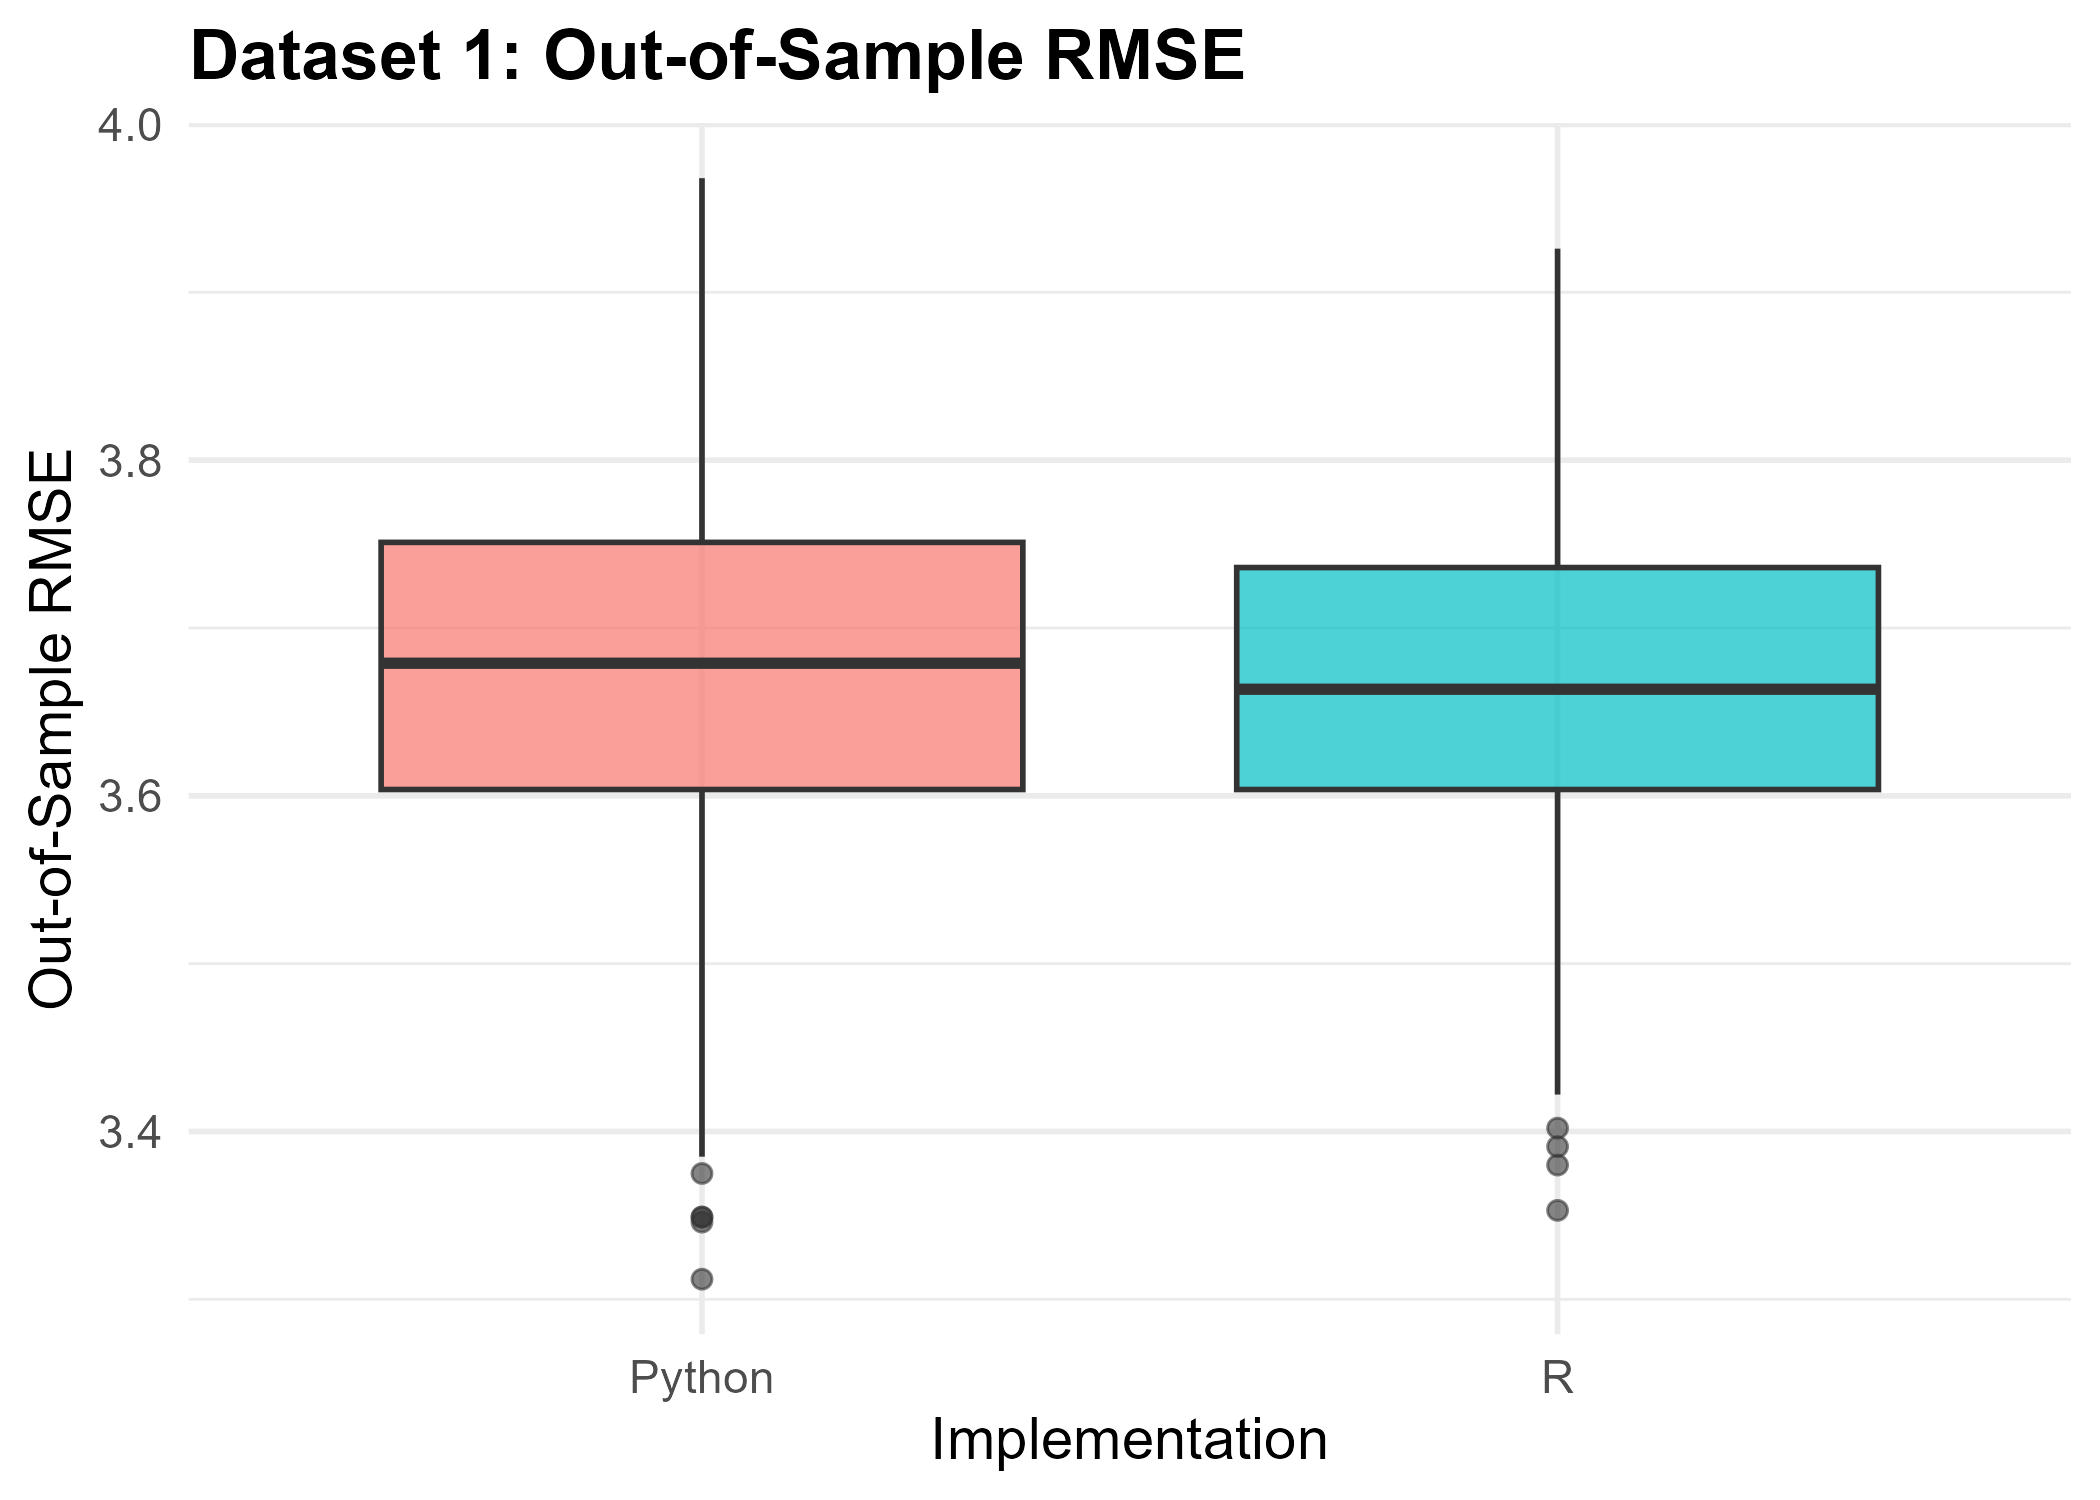
\includegraphics[width=\textwidth]{ormse1.jpg}
    \caption{oRMSE 1}
\end{subfigure}

\vspace{0.3cm}

% Row 2 (Dataset 2)
\begin{subfigure}{0.48\textwidth}
    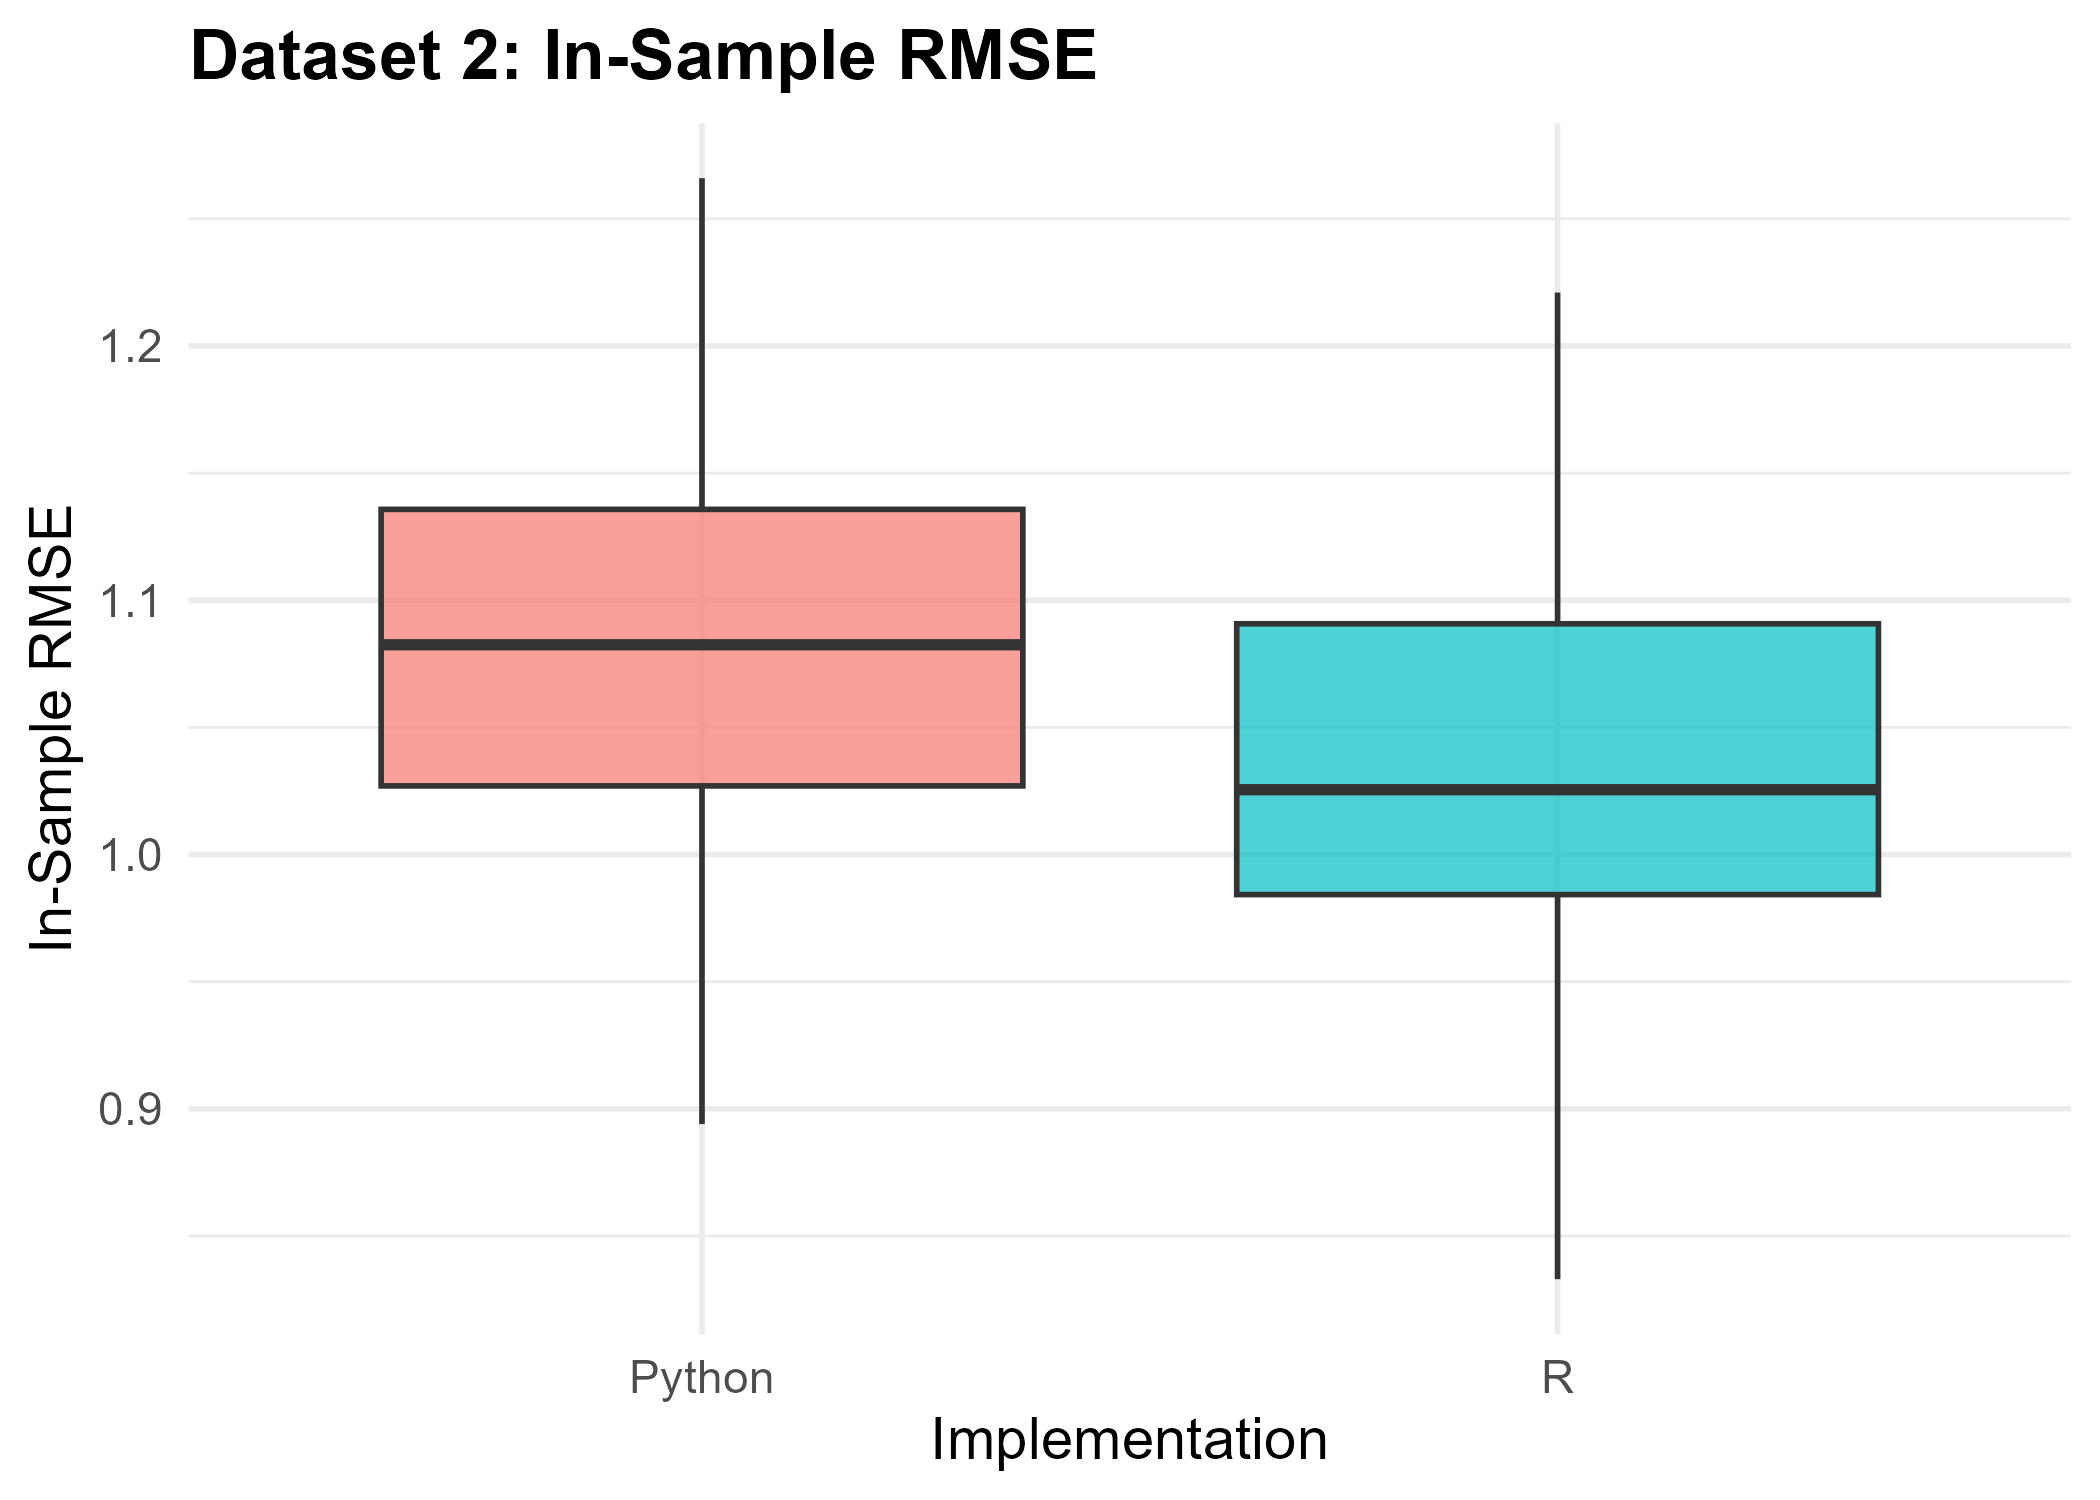
\includegraphics[width=\textwidth]{irmse2.jpg}
    \caption{iRMSE 2}
\end{subfigure}
\begin{subfigure}{0.48\textwidth}
    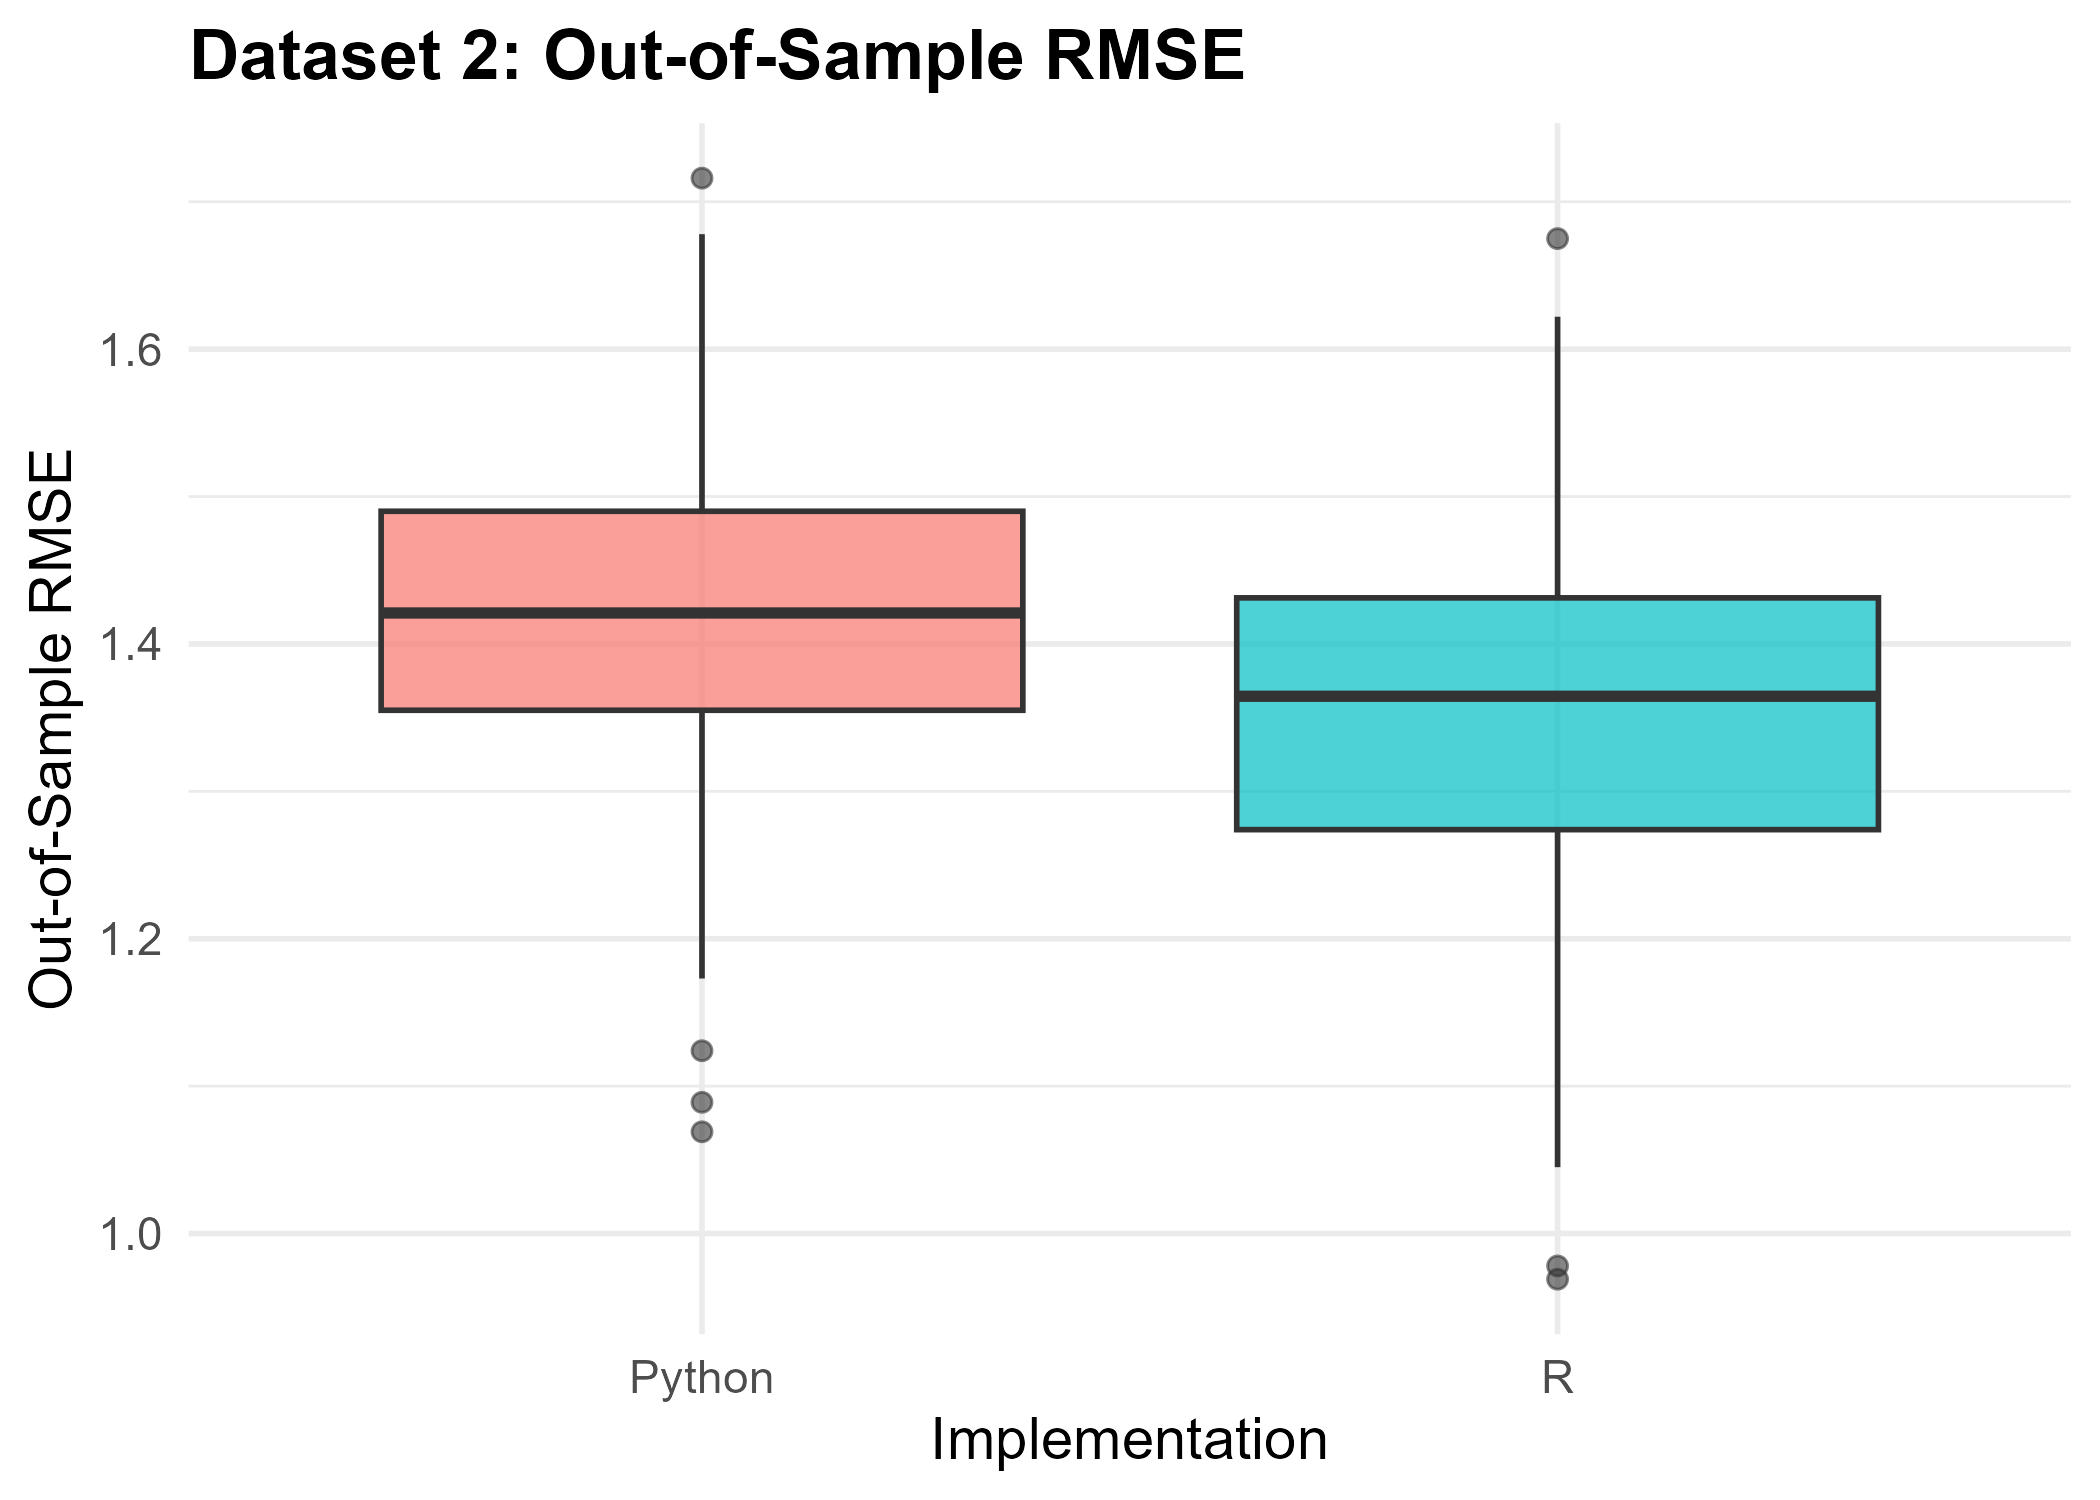
\includegraphics[width=\textwidth]{ormse2.jpg}
    \caption{oRMSE 2}
\end{subfigure}

\vspace{0.3cm}

% Row 3 (Dataset 3)
\begin{subfigure}{0.48\textwidth}
    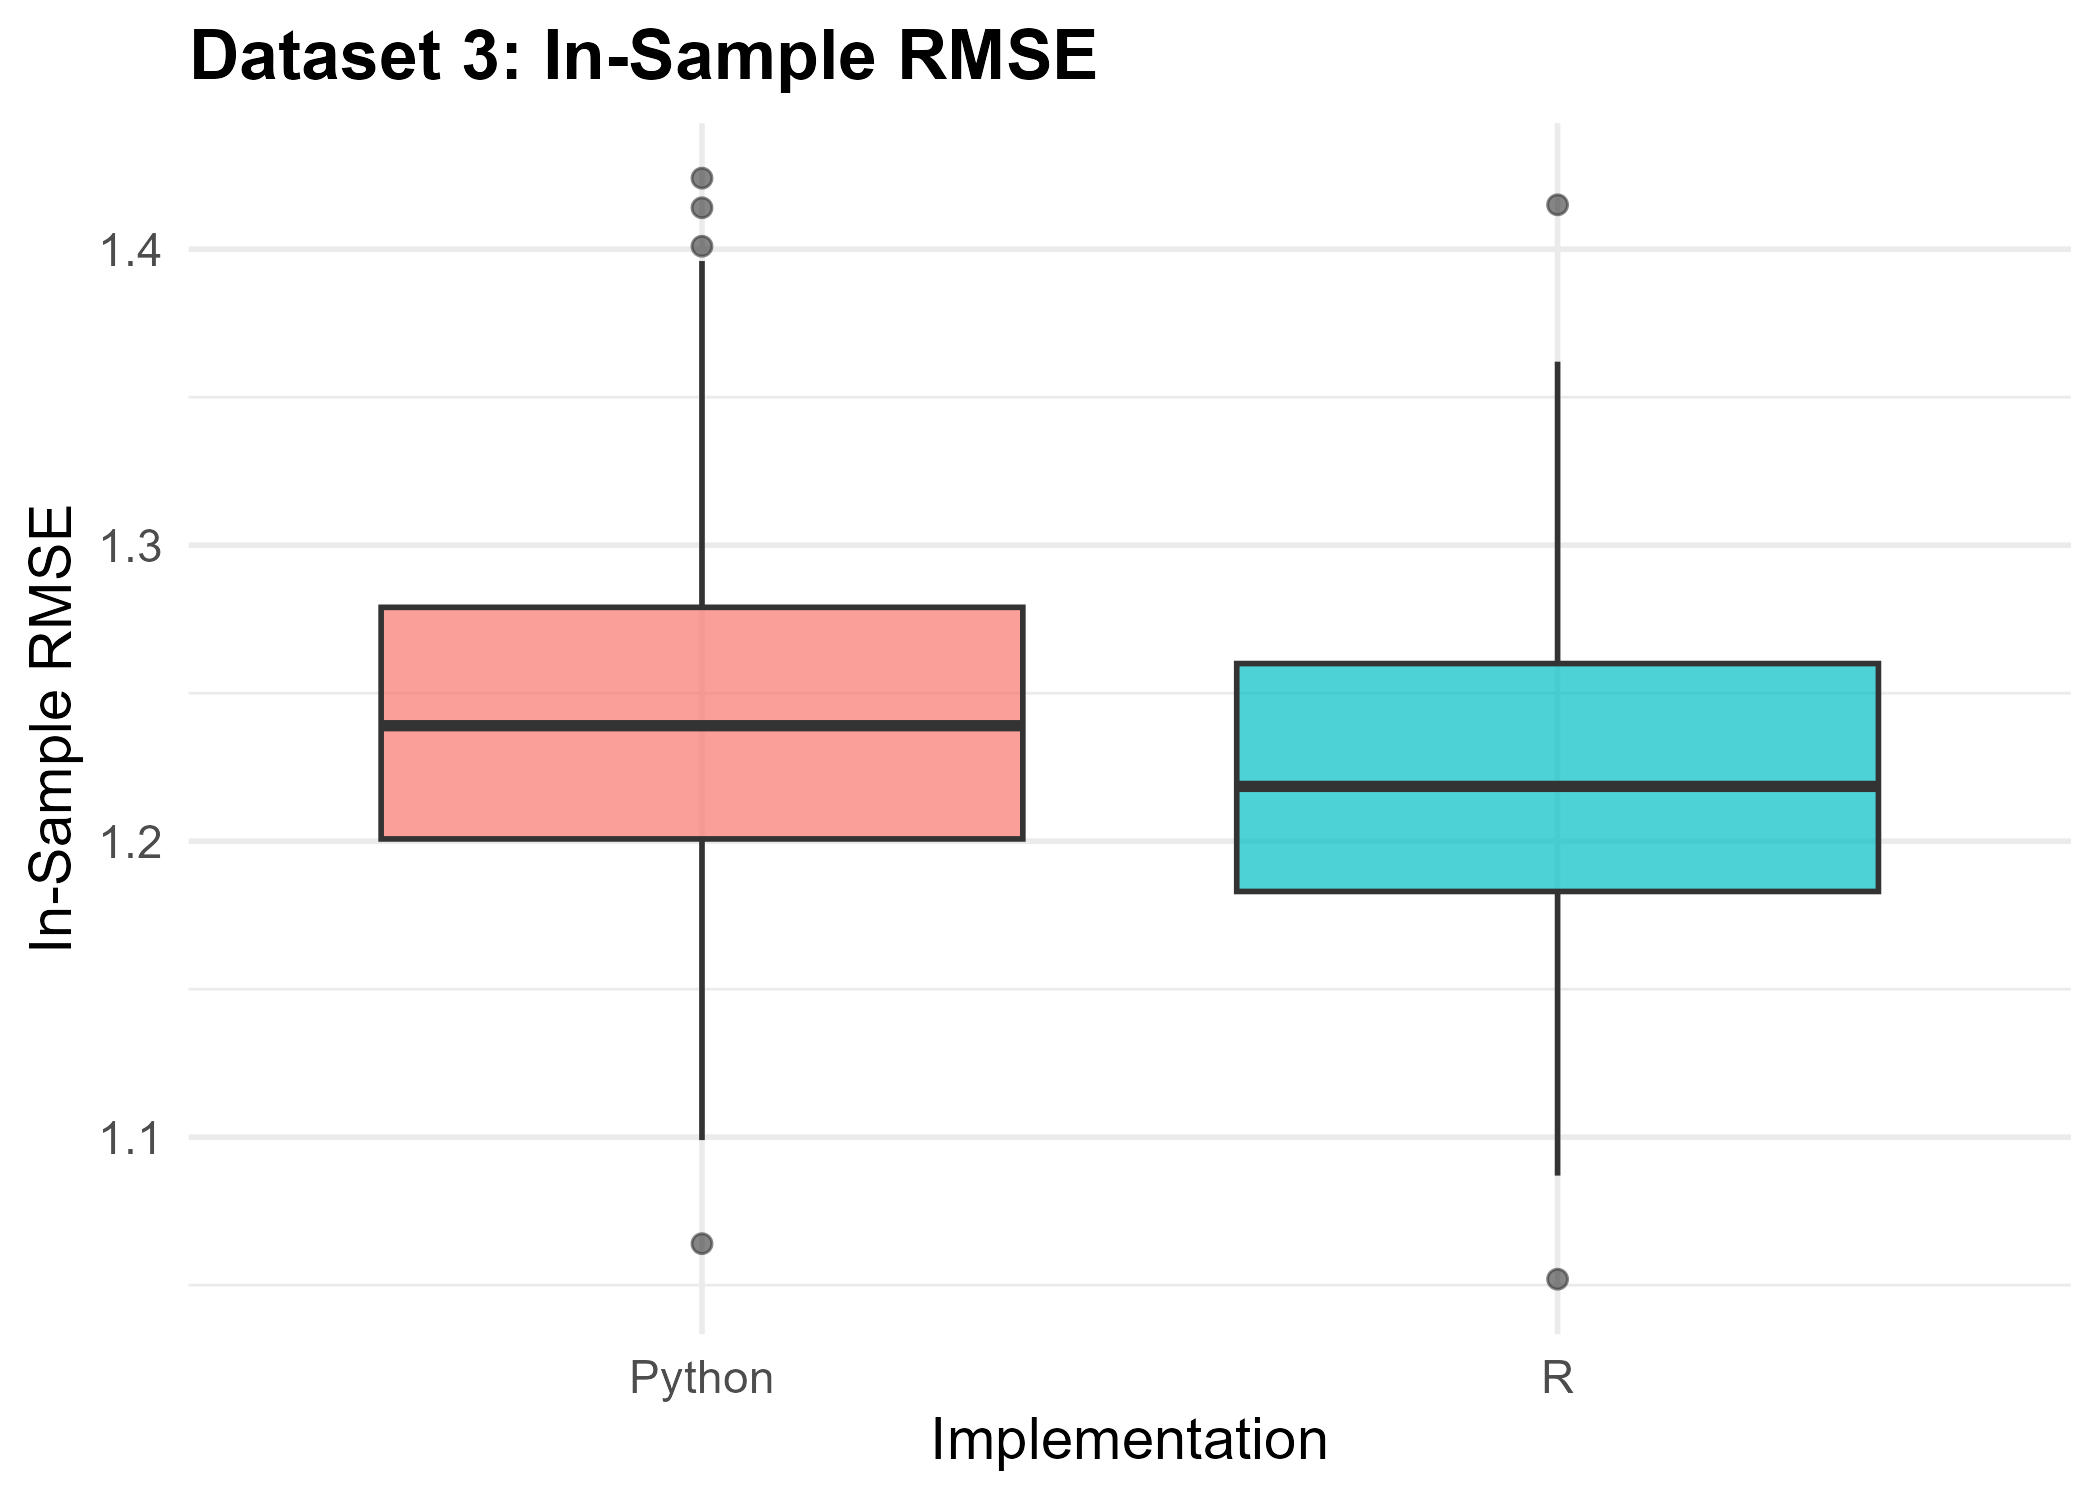
\includegraphics[width=\textwidth]{irmse3.jpg}
    \caption{iRMSE 3}
\end{subfigure}
\begin{subfigure}{0.48\textwidth}
    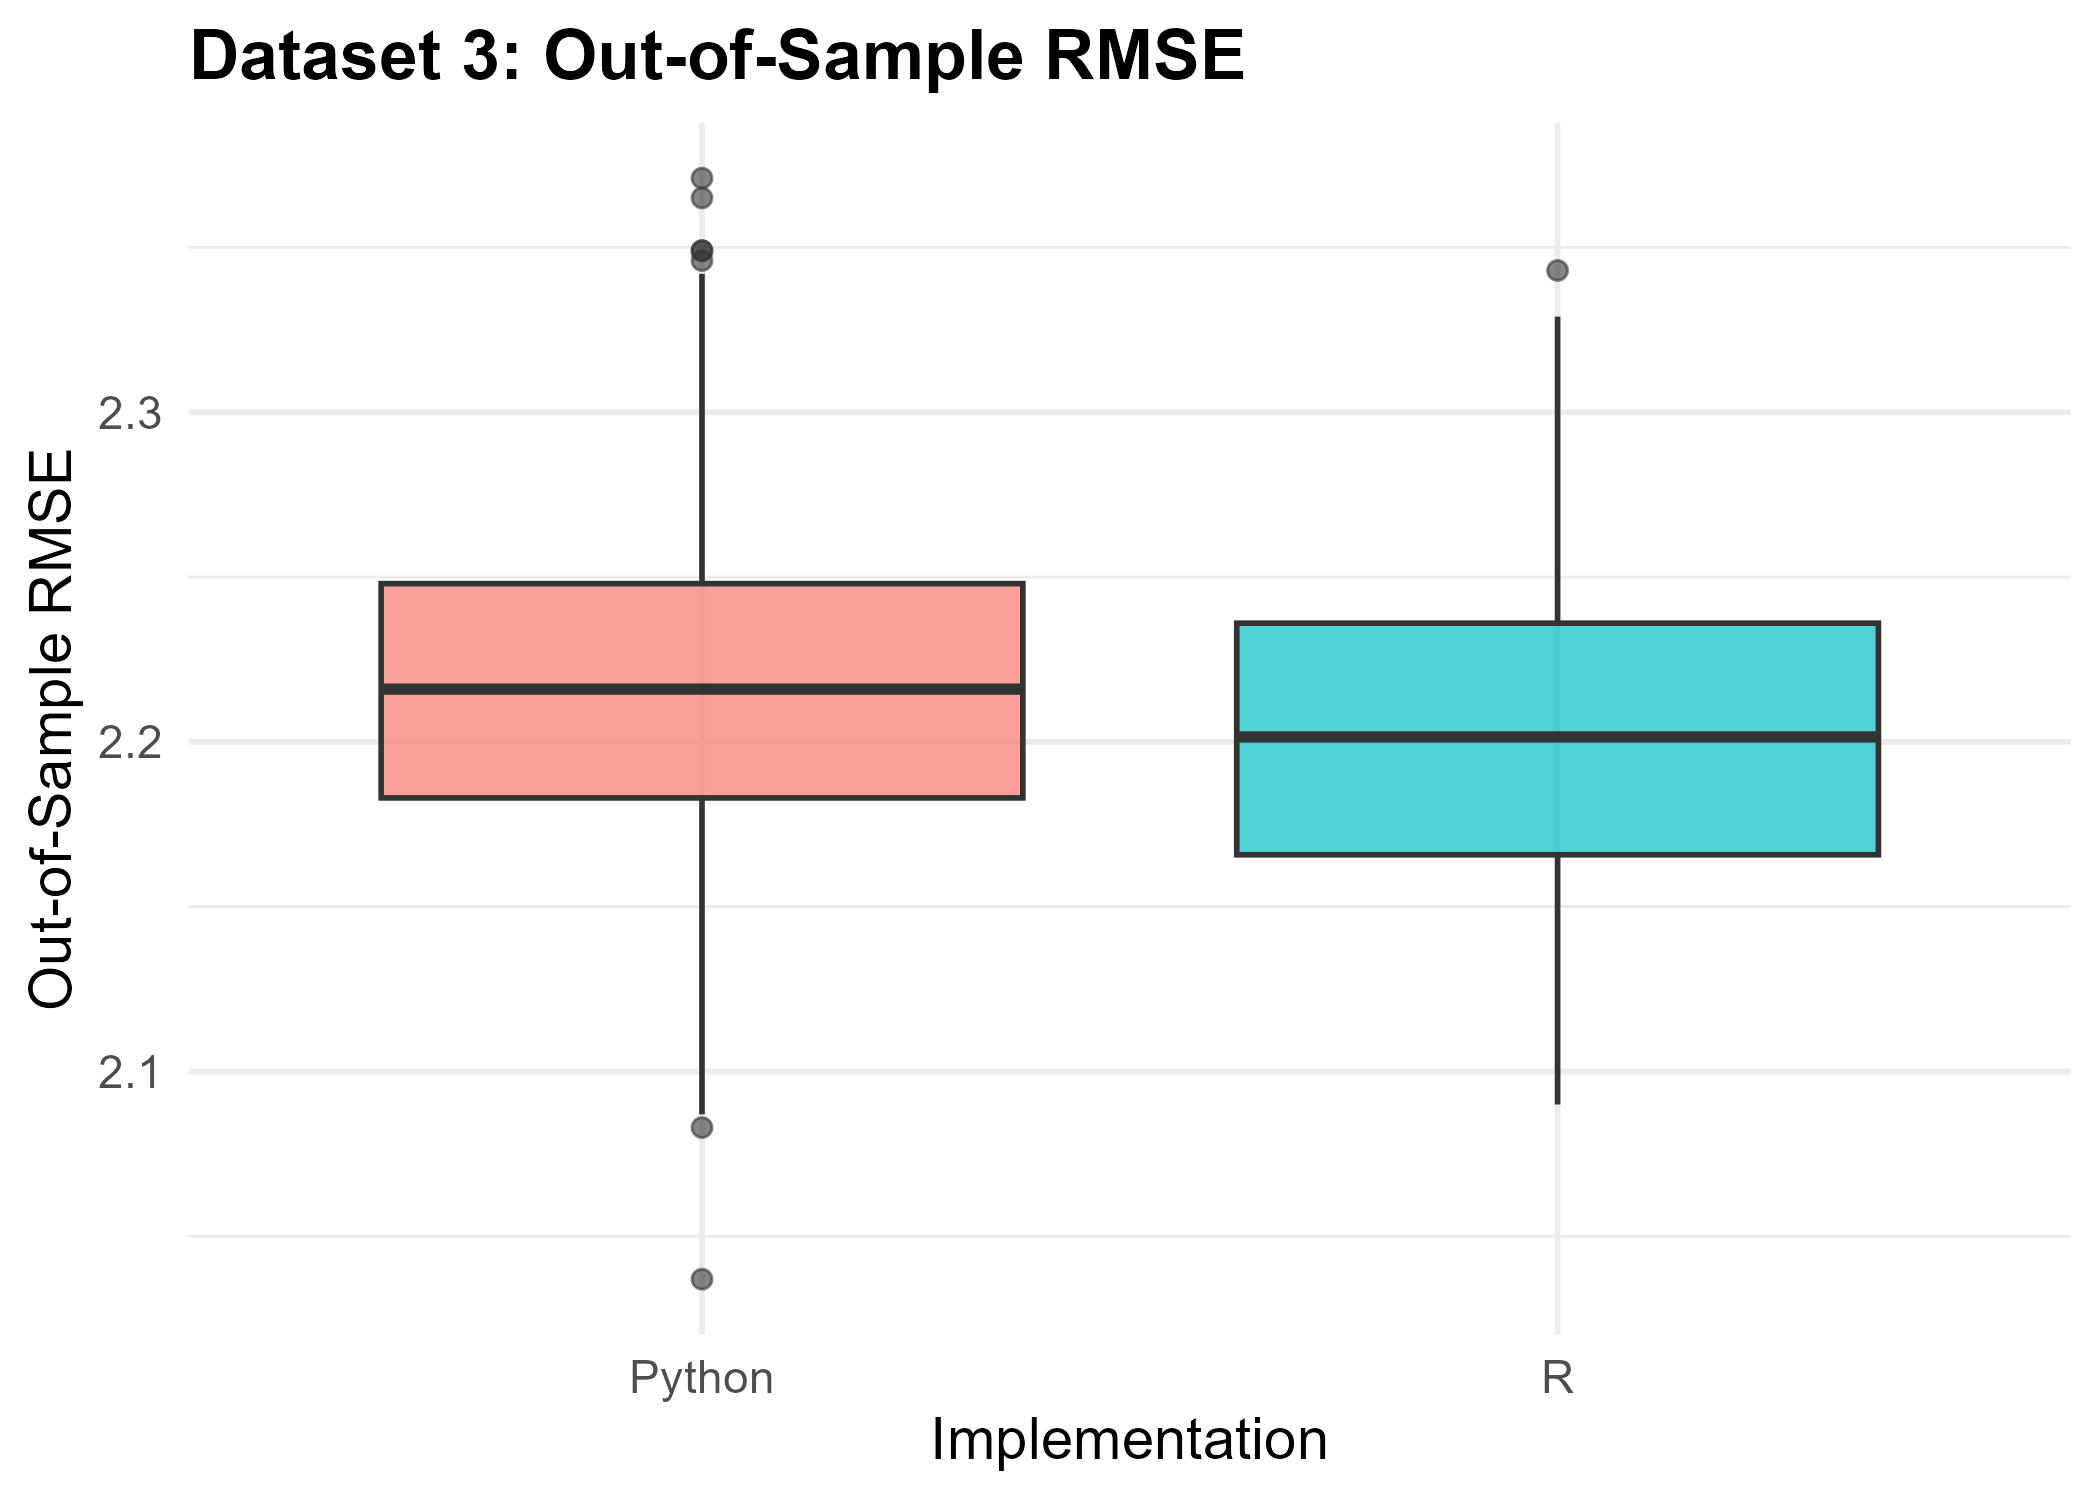
\includegraphics[width=\textwidth]{ormse3.jpg}
    \caption{oRMSE 3}
\end{subfigure}

\vspace{0.3cm}

% Row 4 (Dataset 4)
\begin{subfigure}{0.48\textwidth}
    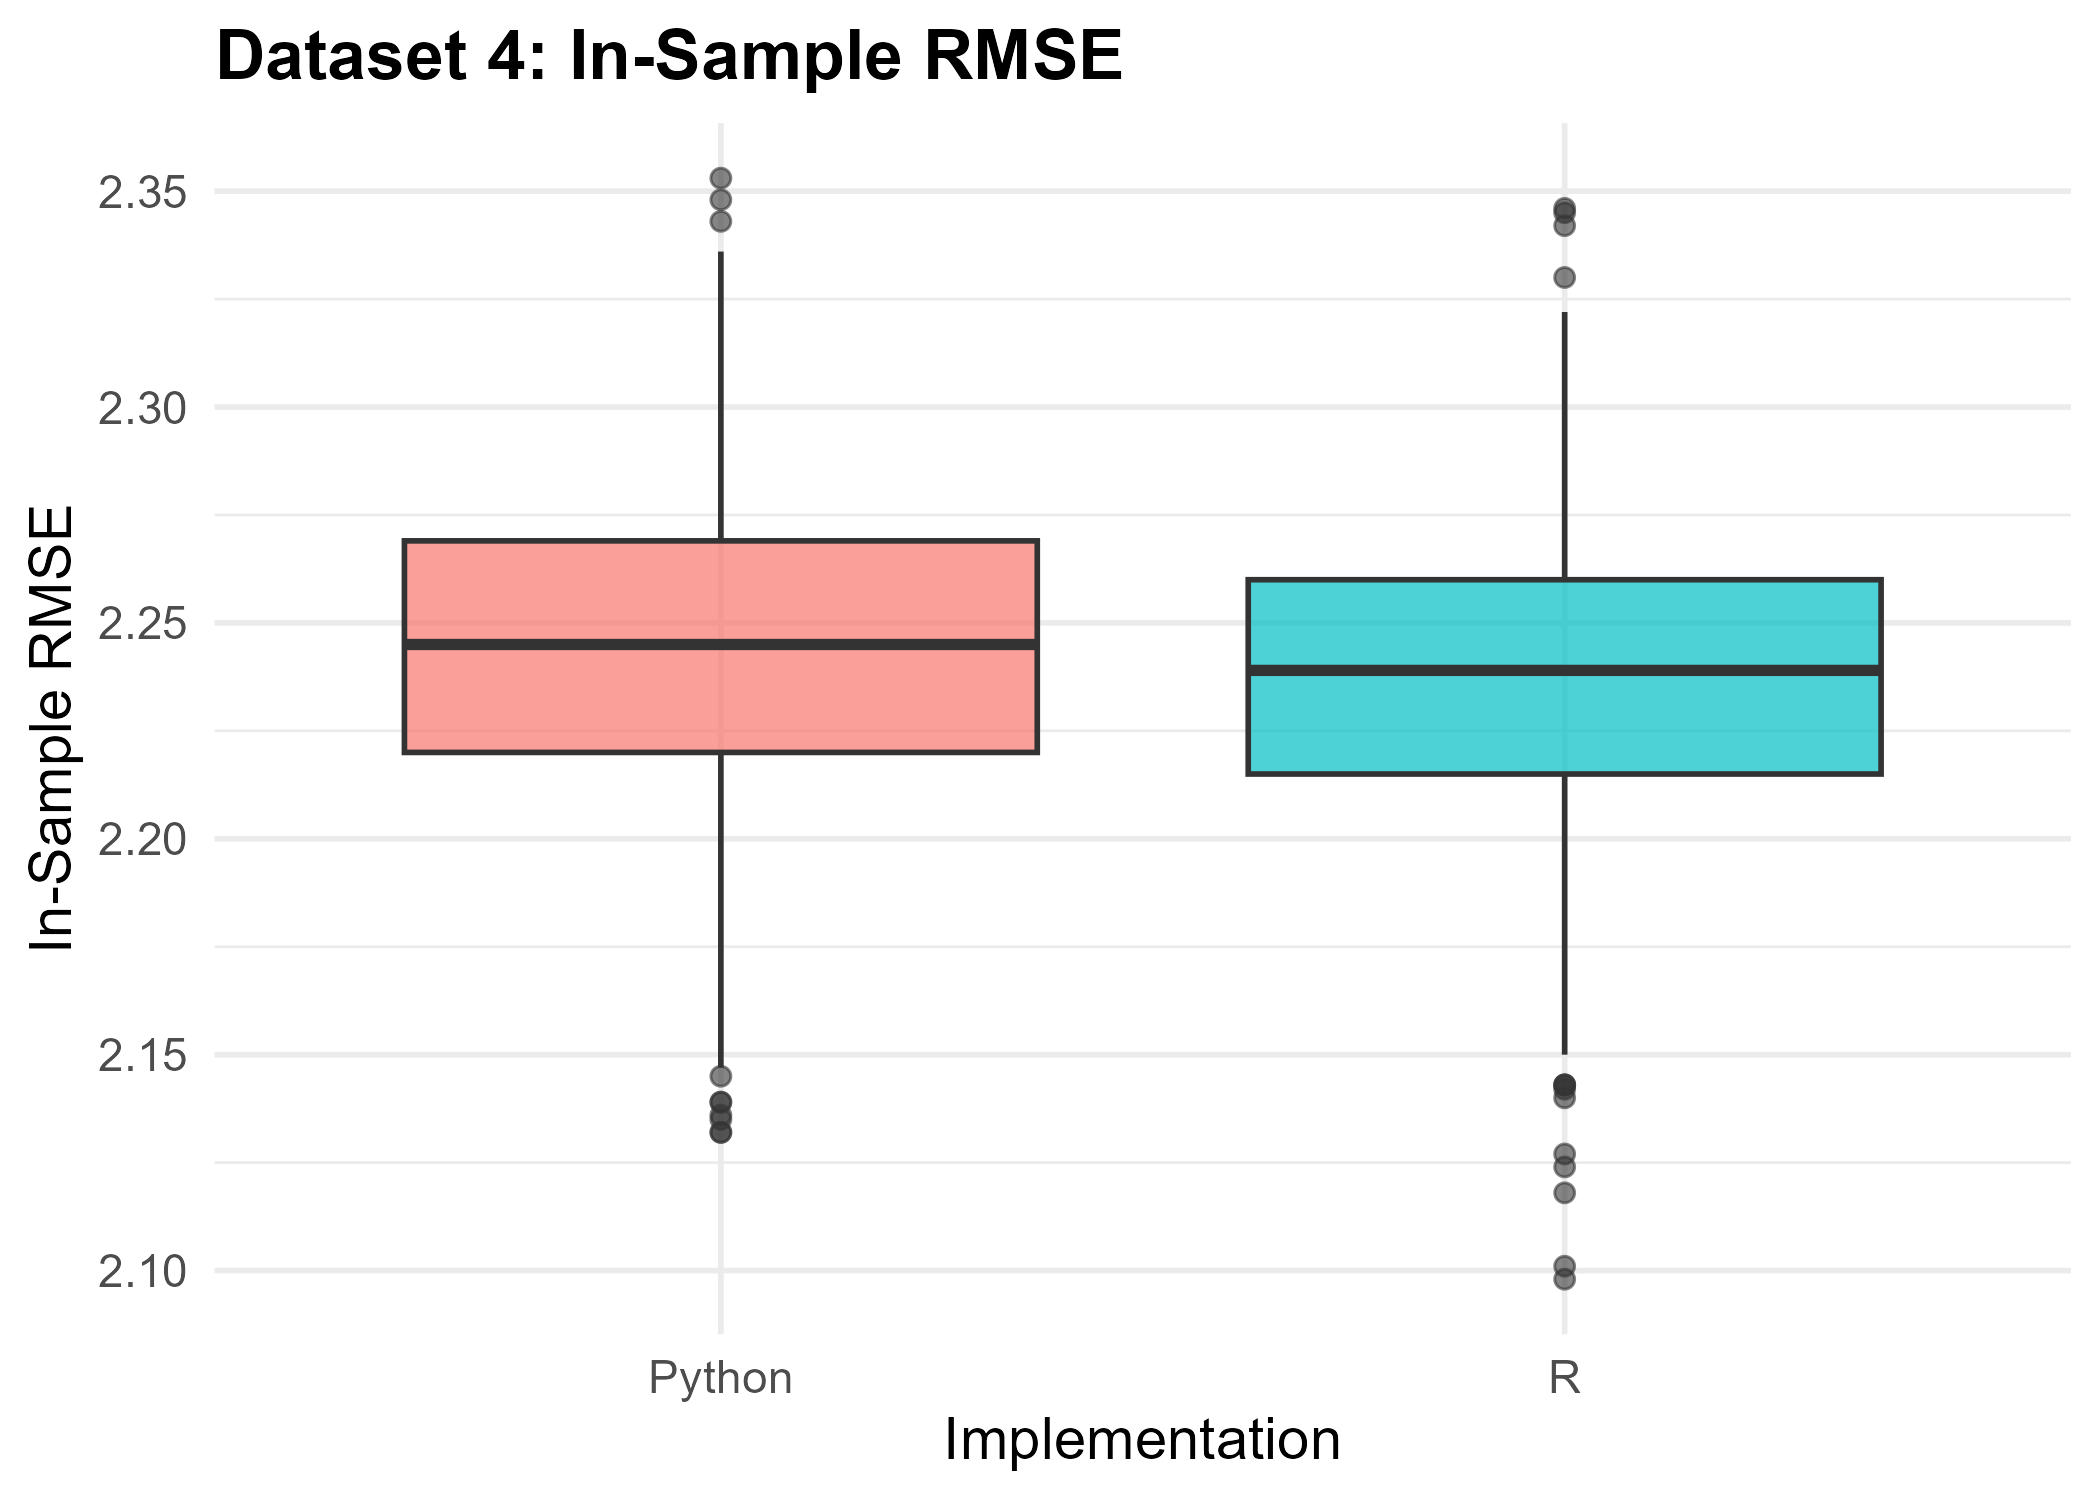
\includegraphics[width=\textwidth]{irmse4.jpg}
    \caption{iRMSE 4}
\end{subfigure}
\begin{subfigure}{0.48\textwidth}
    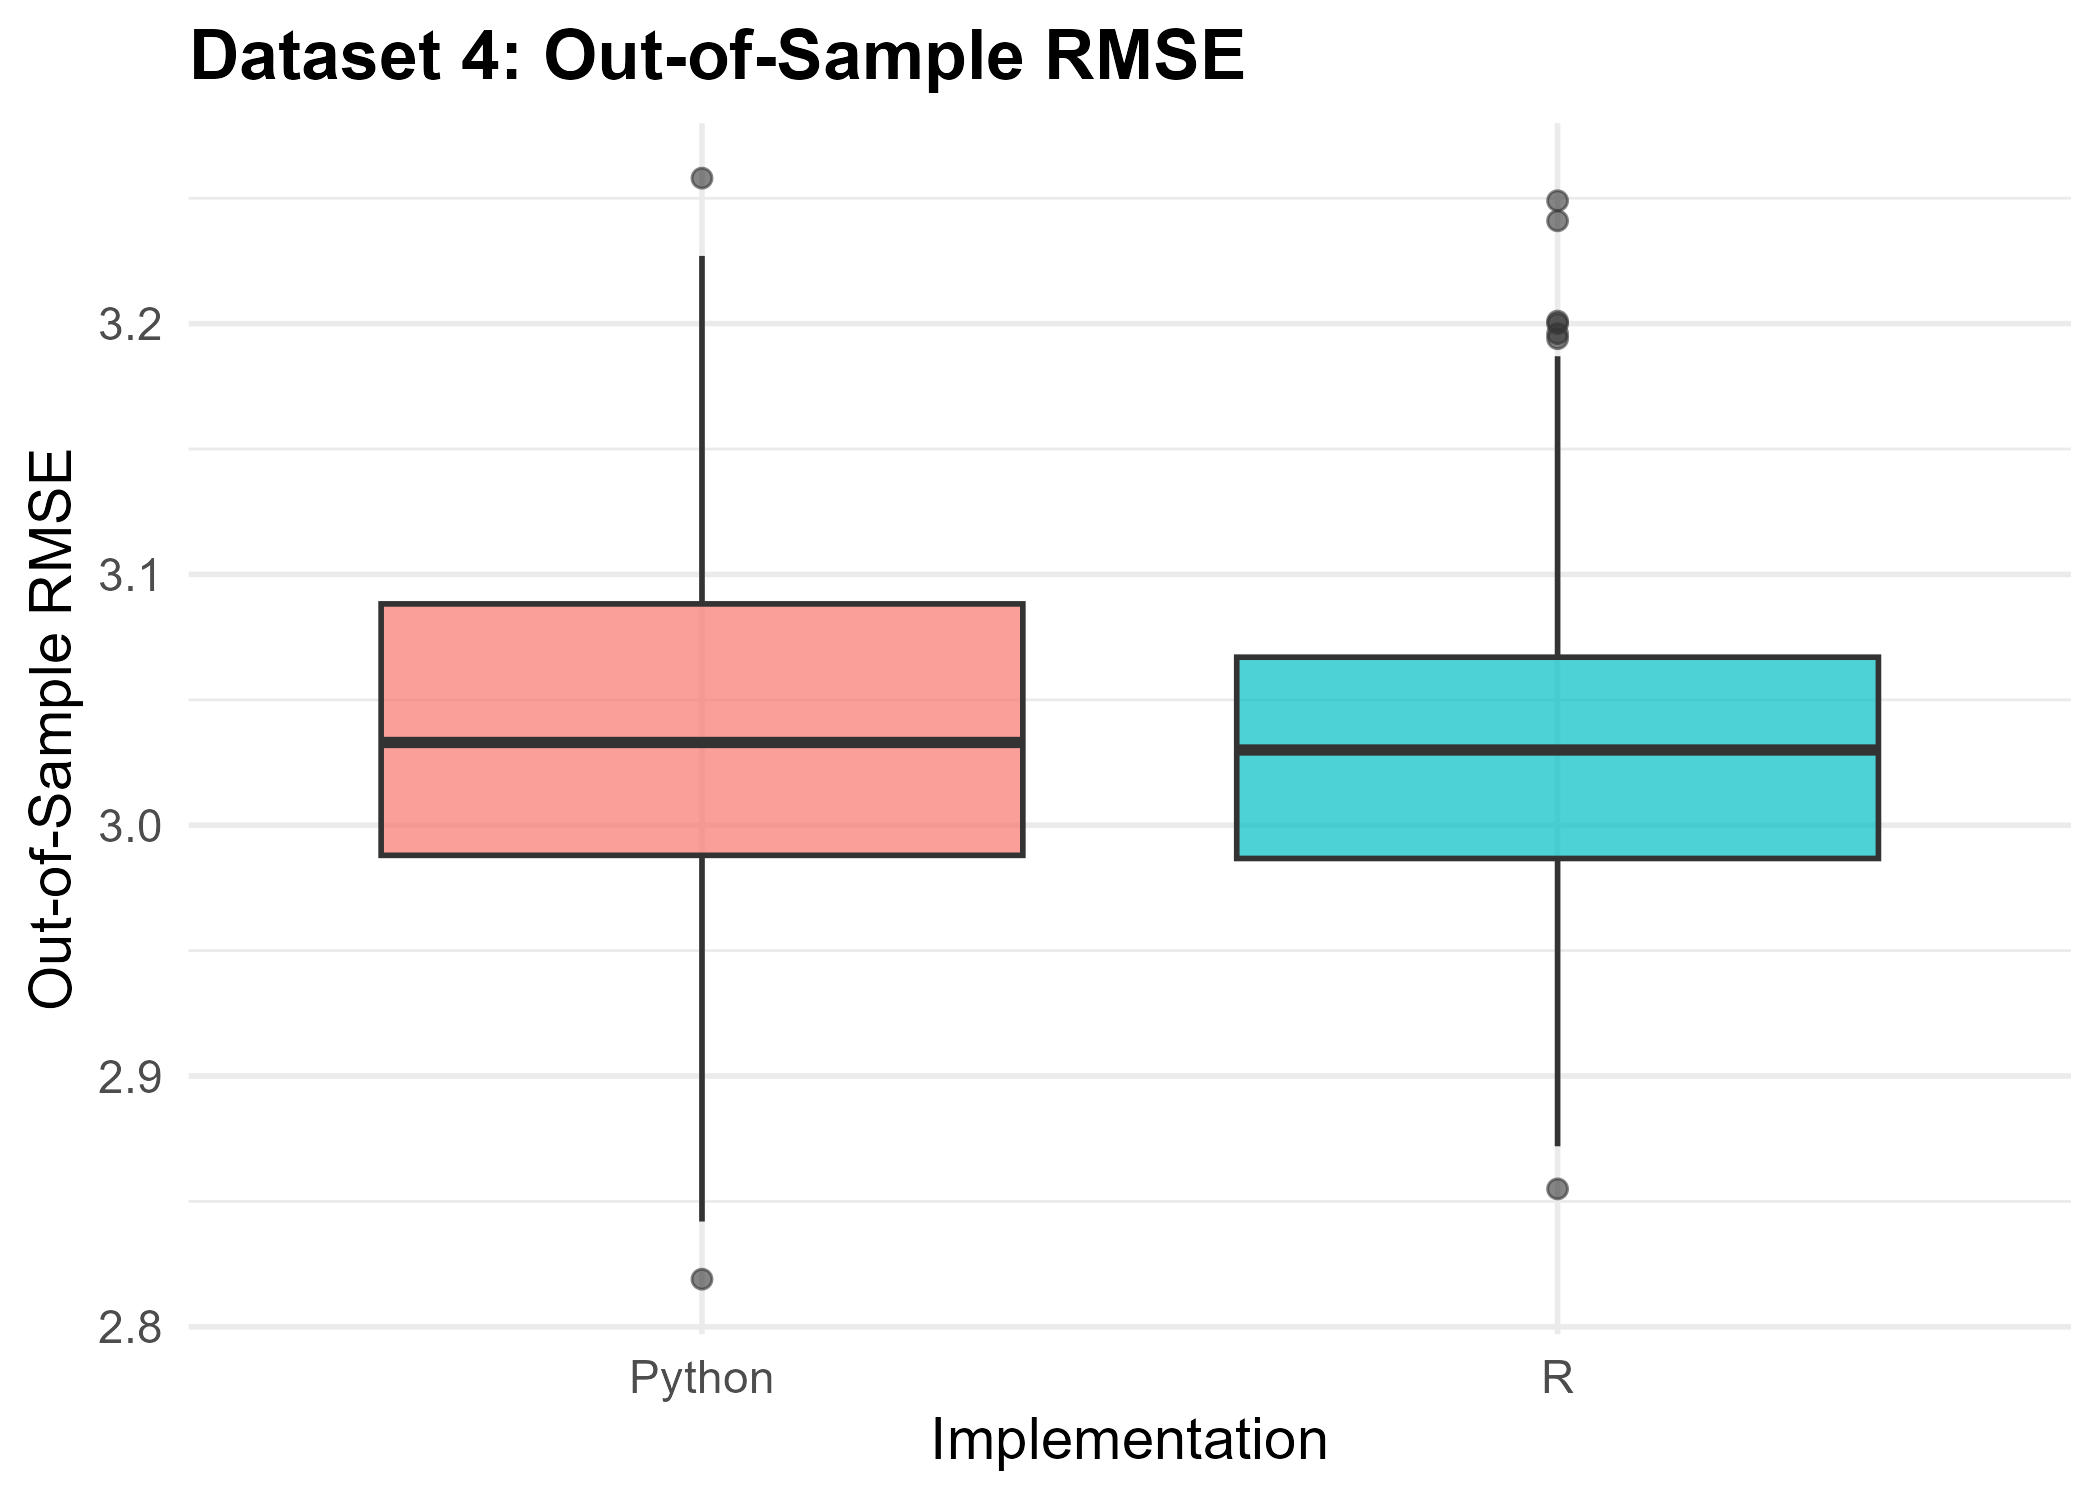
\includegraphics[width=\textwidth]{ormse4.jpg}
    \caption{oRMSE 4}
\end{subfigure}

\caption{In-sample and out-of-sample RMSE across datasets.}
\end{figure}
\newpage
\section{Analysis of results}
\subsection{Fit times}
The mean fit time using Python was lower for all models, and substantially lower for all models, excluding model 3 (spherical). With an average decrease of 22\% in mean fit time using Python, we can certainly conclude that the Python implementation is significantly faster than R at fitting the AddiVortes model using a Euclidean metric.
The standard deviation of fit times using Python was significantly lower for all models, with an average decrease of 73\% when using Python instead of R.
\\
\\
Therefore in terms of both lower and more consistent fit times, Python is superior.
\subsection{Prediction times}
The mean prediction time using Python was significantly lower for all models, with an average decrease of 51\% when using Python instead of R. The standard deviation of fit times using Python was significantly lower for all models, with an average decrease of 77\% when using Python instead of R.
\\
\\
Therefore in terms of both lower and more consistent fit times, Python is superior.
\subsection{In-sample RMSEs}
The mean in-sample RMSE using Python was slightly higher for all models, with an average increase of 2\% when using Python instead of R. The standard deviation of in-sample RMSEs using Python gave mixed results in comparison to R. The standard deviation of in-sample RMSEs on model 1 was significantly higher. This model, representing real world data that could be more unstructured than the synthetic datasets we generated, should be the most significant for us here, where the other differences vary in sign.
\\
\\
Therefore in terms of lower and more consistent in-sample RMSEs, we should take a slight preference for R, with its slightly, but consistently, better mean in-sample RMSEs, and its proficiency for more consistent in-sample RMSEs with the real-world dataset used.
\subsection{Out-of-sample RMSEs}
The mean out-of-sample RMSE using Python gave mixed results in comparison to R. The mean out-of-sample RMSE was almost the same for models 1 and 4, with only a slight increase for model 2. This shows that R also has a slightly lower mean out-of-sample RMSE using a Euclidean metric. On the other hand, the out-of-sample RMSE was significantly lower for model 3 (spherical), with a reduction of 51\% in mean value. The standard deviation of out-of-sample RMSEs using Python was significantly lower for models 2 and 3, with models 1 and 4 having much smaller changes with varying sign. This demonstrates that Python can generate much more consistent out-of-sample RMSEs.
\\
\\
Therefore in terms of out-of-sample RMSEs, it seems that R produces a consistently slightly lower mean, when using the Euclidean metric, however Python seems to be able to produce much more consistent values, and produces a much lower mean out-of-sample RMSE when using the Spherical metric. Hence it is hard to demonstrate any clear preference we should have of either implementation in this regard.
\section{Conclusion}
Given that the results obtained using Python are significantly faster and more consistent, and there is only evidence of a very slight reduction in RMSEs when using R, I would recommend the Python implementation for further use and testing.
\newpage
\appendix
\section{Significance of results using standard errors}
Let $\bar{X}_{f_1}$ be our sample mean fit time for test 1 using R and $\bar{Y}_{f_1}$ be our sample mean fit time for test 1 using Python.
$$
Var(\bar{X}_{f_1}-\bar{Y}_{f_1}) = Var(\bar{X}_{f_1}) + Var( \bar{Y}_{f_1})
$$\\
Note that we are using samples with 106 observations and hence need to use our standard errors, by scaling our standard deviations from tables 2 and 4 by a factor of $\frac{1}{\sqrt{n}}$. We can then calculate the standard error of the difference of the means:
$$
SE(\bar{X}_{f_1}-\bar{Y}_{f_1}) = \sqrt{SE(\bar{X}_{f_1})^2 + SE(\bar{Y}_{f_1})^2}
$$
We divide the difference in the mean values $\bar{X}_{f_1}-\bar{Y}_{f_1}$ by the combined standard error to give z-values for these differences. We will consider z-values over 2 as significant (roughly 95\% significance level). The results of these analyses are below:
\begin{table}[htbp]
\centering
\caption{Fit and prediction standard errors}
\label{tab:fit_pred_ses}
\begin{adjustbox}{width=\textwidth}

\begin{tabular}{l|r|r|r|r|r|r}
\hline
Test & Fit SE (R) & Fit SE (Python) & Pred SE (R) & Pred SE (Python) & Fit SE (Comb) & Pred SE (Comb)\\
\hline
Test 1 & 0.012 & 0.018 & 0.011 & 0.004 & 0.022 & 0.011\\
\hline
Test 2 & 0.002 & 0.006 & 0.003 & 0.002 & 0.006 & 0.003\\
\hline
Test 3 & 0.006 & 0.012 & 0.010 & 0.008 & 0.013 & 0.013\\
\hline
Test 4 & 0.004 & 0.003 & 0.002 & 0.001 & 0.005 & 0.002\\
\hline
\end{tabular}

\end{adjustbox}
\end{table}
\begin{table}[htbp]
\centering
\caption{iRMSE and oRMSE standard errors}
\label{tab:rmse_ses}
\begin{adjustbox}{width=\textwidth}

\begin{tabular}{l|r|r|r|r|r|r}
\hline
Test & iRMSE SE (R) & iRMSE SE (Python) & oRMSE SE (R) & oRMSE SE (Python) & iRMSE SE (Comb) & oRMSE SE (Comb)\\
\hline
Test 1 & 0.003 & 0.003 & 0.010 & 0.011 & 0.005 & 0.015\\
\hline
Test 2 & 0.008 & 0.008 & 0.011 & 0.010 & 0.011 & 0.015\\
\hline
Test 3 & 0.006 & 0.006 & 0.004 & 0.005 & 0.008 & 0.007\\
\hline
Test 4 & 0.004 & 0.004 & 0.006 & 0.007 & 0.005 & 0.009\\
\hline
\end{tabular}

\end{adjustbox}
\end{table}
\begin{table}[htbp]
\centering
\caption{Fit and prediction z-values}
\label{tab:fit_pred_sig}
\begin{adjustbox}{width=\textwidth}

\begin{tabular}{l|r|r|r|r|r|r}
\hline
Test & Fit Diff & Pred Diff & Fit SE (Comb) & Pred SE (Comb) & Fit Diff SEs & Pred Diff SEs\\
\hline
Test 1 & 2.699 & 4.247 & 0.094 & 0.078 & 28.663 & 54.451\\
\hline
Test 2 & 0.492 & 0.714 & 0.027 & 0.015 & 18.417 & 48.470\\
\hline
Test 3 & 0.267 & 0.392 & 0.037 & 0.029 & 7.308 & 13.636\\
\hline
Test 4 & 0.214 & 0.288 & 0.009 & 0.005 & 24.084 & 56.064\\
\hline
\end{tabular}

\end{adjustbox}
\end{table}
\begin{table}[htbp]
\centering
\caption{iRMSE and oRMSE z-values}
\label{tab:rmse_sig}
\begin{adjustbox}{width=\textwidth}

\begin{tabular}{l|r|r|r|r|r|r}
\hline
Test & iRMSE.Diff & oRMSE.Diff & iRMSE.SE.Comb. & oRMSE.SE.Comb. & iRMSE.Diff.SEs & oRMSE.Diff.SEs\\
\hline
Test 1 & 0.015 & 0.000 & 0.005 & 0.014 & 3.114 & 0.002\\
\hline
Test 2 & 0.051 & 0.045 & 0.011 & 0.022 & 4.573 & 2.045\\
\hline
Test 3 & 0.021 & 2.314 & 0.007 & 0.055 & 3.156 & 41.907\\
\hline
Test 4 & 0.007 & 0.015 & 0.005 & 0.009 & 1.446 & 1.669\\
\hline
\end{tabular}

\end{adjustbox}
\end{table}
\newpage
\textit{Note for the purposes of this analysis we will ignore test 3, the results of which are the artefact of a bug in the code}\\
\\
Clearly, all of the differences in fit times and prediction times are highly significant, with Python having the significantly lower times for both. Some of the iRMSE and oRMSE differences are significant, but there are also some insignificant results, especially within oRMSE where significances were significantly lower than in iRMSE.\\
\\
Therefore, since there is limited evidence to suggest the R implementation has lower oRMSEs, and there is strong evidence to suggest the Python implementation has faster fit and prediction times, I would suggest Python to be used, this agrees with our previous conclusion.
\end{document}